\documentclass[11pt,letterpaper]{article}
\usepackage[margin=1in,headheight=15pt]{geometry}
\usepackage[T1]{fontenc}
\usepackage[utf8]{inputenc}
\usepackage{lmodern}
\usepackage{microtype}
\usepackage{amsmath,amssymb,amsthm,mathtools}
\usepackage{booktabs,longtable,tabularx,array,multirow}
\usepackage{enumitem}
\usepackage{xcolor}
\usepackage{listings}
\usepackage{tikz}
\usetikzlibrary{arrows.meta,positioning,fit,calc,shapes.geometric}
\usepackage{fancyhdr}
\usepackage{hyperref}
\usepackage[nameinlink,noabbrev]{cleveref}
\usepackage{url}
\usepackage{csquotes}

\definecolor{darcblue}{RGB}{28,75,121}
\definecolor{darcteal}{RGB}{25,110,105}
\definecolor{darcgray}{RGB}{245,247,249}
\definecolor{darcred}{RGB}{145,45,45}
\hypersetup{
  colorlinks=true,
  linkcolor=darcblue,
  citecolor=darcteal,
  urlcolor=darcblue,
  pdftitle={DARC-iPRA: Demand-Aware Residualizing Compilation for Intuitionistic Primitive Recursive Arithmetic},
  pdfauthor={OpenAI},
  pdfsubject={A general framework for compiling finitary mathematics into iPRA}
}
\pagestyle{fancy}
\fancyhf{}
\fancyhead[L]{DARC-iPRA}
\fancyhead[R]{Demand-aware proof compilation}
\fancyfoot[C]{\thepage}
\setlength{\parindent}{0pt}
\setlength{\parskip}{0.55em}
\setlength{\emergencystretch}{2em}
\setlist{nosep,leftmargin=2em}
\setcounter{tocdepth}{2}

\lstdefinestyle{darc}{
  basicstyle=\ttfamily\small,
  backgroundcolor=\color{darcgray},
  frame=single,
  rulecolor=\color{black!15},
  breaklines=true,
  columns=fullflexible,
  keepspaces=true,
  showstringspaces=false,
  aboveskip=0.8em,
  belowskip=0.8em
}
\lstset{style=darc}

\newtheorem{theorem}{Theorem}[section]
\newtheorem{lemma}[theorem]{Lemma}
\newtheorem{proposition}[theorem]{Proposition}
\newtheorem{corollary}[theorem]{Corollary}
\newtheorem{definition}[theorem]{Definition}
\newtheorem{remark}[theorem]{Remark}
\newtheorem{example}[theorem]{Example}
\newtheorem{obligation}[theorem]{Residual obligation}

\newcommand{\iPRA}{\mathrm{iPRA}}
\newcommand{\PRAAx}{\mathsf{PRAAx}}
\newcommand{\Prf}{\mathsf{Prf}}
\newcommand{\DARC}{\mathsf{DARC}}
\newcommand{\Contract}{\mathsf{Contract}}
\newcommand{\Res}{\mathsf{Res}}
\newcommand{\Guard}{\mathsf{Guard}}
\newcommand{\Cert}{\mathsf{Cert}}
\newcommand{\Prec}{\mathsf{Prec}}
\newcommand{\Bool}{\mathbb{B}}
\newcommand{\Nat}{\mathbb{N}}
\newcommand{\seq}[2]{#1\;\vdash_{\PRAAx}\;#2}
\newcommand{\join}{\mathbin{\sqcup}}
\newcommand{\meet}{\mathbin{\sqcap}}
\newcommand{\cl}{\operatorname{cl}}
\newcommand{\rank}{\operatorname{rk}}
\newcommand{\monusop}{\mathbin{\dot{-}}}
\newcommand{\code}[1]{\texttt{#1}}
\newcommand{\pathcode}[1]{\path{#1}}
\newcommand{\status}[1]{\textsf{#1}}

\title{\textbf{DARC-iPRA}\\[0.35em]
\Large Demand-Aware Residualizing Compilation for\\
Intuitionistic Primitive Recursive Arithmetic}
\author{Research artifact prepared by OpenAI}
\date{16 November 2026\\
\small Repository baseline: \texttt{2ef31aa3e313d792df6b63bb28babfe48e1f982e}}

\begin{document}
\maketitle

\begin{abstract}
This report develops a general method for translating fixed, finite,
quantitative mathematical arguments into the ordinary object-theory judgment
\(\Prf\;\PRAAx\;\Gamma\;\varphi\) used by the ProveIt formalization of
intuitionistic primitive recursive arithmetic.  The central device is a single
finite product-lattice analysis whose least prefixed point records, at once,
which certificate fields must escape local scope, which approximation
precisions are demanded, which guards or apartness margins are necessary, and
which unproved quantitative producers must remain as explicit residual
hypotheses.  This demand state prunes and specializes the proof graph before
object-proof assembly.  Local noncanonical witnesses are eliminated by
existential elimination; public named witnesses are canonicalized only when
needed, using checked bounded search; fixed bounded formulas are compiled to
primitive-recursive truth bits and finite strategy certificates; loops are
normalized to quantifier-free trace invariants; and finite relational witness
problems are solved by backward viability rather than incompatible independent
choices.

The report proves stabilization and leastness of the demand analysis, the
open-contract/sequent equivalence, certificate escape and residualization
theorems, bounded reflection and strategy soundness schemas, trace and
viability schemas, and a global conditional compilation theorem.  It also
isolates genuine barriers: no total universal evaluator is assumed, no
infinite path follows from horizonwise existence, no regular name follows
without a tail modulus, and no ordered root or eigenvector is selected through
collisions.  A source-oriented Lean kernel, dependency-ordered Lean
blueprints, exact finite reference algorithms, tests, and a machine-readable
plan schema accompany the paper.  No new Lean-kernel-checked theorem is
claimed by this artifact.
\end{abstract}

\begin{center}
\fbox{\parbox{0.92\textwidth}{
\textbf{Verification status.}
The mathematical arguments below are complete at the human-proof level for
the stated generic conditional schemas.  The small Lean structural kernel has
no placeholders but was not elaborated in this runtime.  The larger Lean files
are blueprints with explicit milestones.  Python tests validate finite
metalevel algorithms only; they are not proofs in \(\iPRA\).
}}
\end{center}

\tableofcontents
\clearpage

\section{Executive overview}
\label{sec:executive}

The working problem is not merely to encode one more theorem in arithmetic.
It is to build a reusable route from a broad class of mathematical arguments
to a literal derivation in the ordinary ProveIt judgment
\[
  \Gamma \vdash_{\PRAAx} \varphi,
\]
while respecting the severe but mathematically useful discipline of
intuitionistic primitive recursive arithmetic.  In particular, every function
used in the object language must be primitive recursive, induction is
available only for quantifier-free formulas, and existential information must
be handled constructively rather than extracted by an unrestricted appeal to
choice.

The repository already contains many of the ingredients needed for such a
route.  The ordinary calculus has substitution, weakening, simultaneous cut,
existential elimination, equality transport, and quantifier-free induction.
The checked arithmetic library contains order, bounded search, pairing,
simultaneous recursion, finite sums and products, division with remainder,
gcd, and several higher-level proof patterns.  The checked bridge transports
closed and open sequents to the Foundation presentation used by several
applications.  The difficult part is now architectural: how should a large,
heterogeneous, partly quantitative proof be organized so that only the
resources genuinely needed by a requested conclusion survive into the final
theorem?

\subsection{The new organizing invariant}

DARC answers this question by assigning each fixed proof plan a finite product
of chains
\[
  L = \prod_{r\in R} \{0,1,\ldots,c_r\}.
\]
The coordinates are not all of one kind.  They include:
\begin{enumerate}
  \item public query coordinates, indicating which outputs are requested;
  \item certificate-liveness coordinates, indicating which fields of an
        internal witness must escape its local existential scope;
  \item precision coordinates, recording the finite accuracy required from
        approximation subroutines;
  \item guard coordinates, such as denominator apartness, root separation, a
        spectral gap, or finite-net coverage;
  \item residual coordinates, indicating quantitative producer theorems that
        have not been supplied and must therefore remain hypotheses of the
        compiled endpoint;
  \item optional backend coordinates, when a consumer requires a translated
        vocabulary or a particular published presentation.
\end{enumerate}
Each local proof node contributes a monotone backward transfer rule.  Starting
from the public query, DARC iterates
\[
  d_{s+1}=d_s\join F(d_s).
\]
Because the lattice is a finite product of chains, every strict step increases
the sum of the coordinates.  Hence the process stabilizes after at most
\(\sum_r c_r\) strict steps.  Its value is the least prefixed point above the
query seed.  The word ``least'' is relative to the declared transfer summaries:
DARC does not claim that no cleverer proof could use fewer resources.  It does
prove that no state satisfying those summaries can omit a resource retained by
the analysis.

This one invariant subsumes several analyses that otherwise tend to drift
apart.  A branch label is retained exactly when the public result names that
branch.  A tail modulus is exposed exactly when the requested precision reaches
a node whose proof needs it.  A quantitative nonzero margin is requested only
when a live operation divides or pivots.  A height bound is absent from a
purely observational theorem but appears if the theorem asks for a complete
list of witnesses.  Dead nodes and dead certificate fields are erased before
proof assembly.

\subsection{Compilation in two levels}

The framework deliberately separates two levels.

\paragraph{Metalevel specialization.}
Lean or another trusted generator traverses one fixed finite proof plan,
computes its demand closure, specializes every fixed bounded formula to
concrete primitive-recursive symbols, and constructs an explicit derivation
term.  This traversal may recurse on the plan's syntax because it happens in
the metatheory.

\paragraph{Object-level proof.}
The generated theorem is an ordinary \(\Prf\;\PRAAx\) derivation.  It does not
quantify over proof plans, program codes, or formula syntax.  It uses only the
specific primitive-recursive symbols generated for that plan, their defining
equations, successor axioms, intuitionistic logic, and quantifier-free
induction.

This distinction is the clean resolution of the universal-evaluator problem.
There is no primitive-recursive total evaluator for all primitive-recursive
programs with their unbounded running time.  DARC needs none.  It produces a
new fixed symbol for each fixed program, exactly as the ordinary \(\iPRA\)
language permits.

\subsection{Three certificate export modes}

Every internal certificate is classified after demand closure.

\begin{description}
  \item[Sealed.] The public result is independent of the certificate.  A local
  producer \(\Gamma\vdash\exists c\,V(c)\) and a consumer
  \(V(c),\Gamma\vdash\Phi\) are joined by existential elimination.  No
  canonical certificate is constructed.

  \item[Observed.] The result depends only on an invariant observation
  \(O(c)\), and the proof establishes that all valid certificates yield the
  same observation, or yield observations related by a specified tolerance.
  The certificate remains hidden; only the stable observation escapes.

  \item[Named.] The public statement really names a witness or code.  DARC
  requires a finite search bound and a primitive-recursive validity bit, then
  uses the checked least-search theorem to select the least valid code.  The
  expense and additional hypotheses of canonicalization occur only in this
  mode.
\end{description}
This trichotomy prevents a common source of unnecessary strength: choosing a
canonical representative merely because an external proof assistant happens
to store one.

\subsection{The main conditional theorem}

Informally, the global theorem proved in \cref{sec:global} is the following.

\begin{theorem}[DARC compilation, informal]
Let \(P\) be a fixed finite proof plan whose cyclic computational components
have been isolated as bounded loop blocks.  Suppose that:
\begin{enumerate}
  \item every demand transfer is monotone and sound for its local node;
  \item every active acyclic node has an ordinary open derivation from the
        conclusions of its dependencies and the residual formulas selected by
        the final demand;
  \item every loop block has a quantifier-free invariant with base and step
        derivations;
  \item every retained named certificate has a finite bound and a reflected
        validity bit;
  \item every retained residual formula is either left as a hypothesis or is
        supplied by an ordinary derivation.
\end{enumerate}
Then the DARC algorithm terminates and constructs an ordinary derivation
\[
  \Res(P,d^*)\vdash_{\PRAAx}\Phi_P,
\]
where \(d^*\) is the least demand state above the public query.  Supplying any
subset of the residual producers eliminates the corresponding hypotheses by
simultaneous cut.  Dead certificates, guards, precisions, and proof nodes do
not occur in the generated endpoint.
\end{theorem}

The theorem is conditional in the right way.  It does not hide deep mathematics
inside a compiler.  For example, a general effective height bound for a
Diophantine problem remains a producer theorem.  Once such a theorem is
provided, the same compiler can use it; until then, the endpoint states it
exactly as a residual.

\subsection{What the framework resolves and what it refuses to blur}

DARC resolves the routine but pervasive difficulties of context management,
finite bounded quantification, proof-local witness handling, precision
bookkeeping, and finite relational compatibility.  It also makes several
negative results operational:
\begin{itemize}
  \item finite-horizon compatible paths do not by themselves produce an
        infinite path;
  \item metastable finite windows do not by themselves produce a convergence
        rate;
  \item a coherent approximation chain is not automatically a regular real
        name without a tail modulus;
  \item a multiset of colliding roots does not support continuous ordered
        labels without a separation condition;
  \item qualitative finiteness does not produce an effective search cutoff.
\end{itemize}
Instead of treating these as failures, the framework turns the missing data
into typed residual interfaces.  This is essential for trustworthy use of a
weak constructive arithmetic.

\section{Repository audit and design constraints}
\label{sec:audit}

The framework was designed against the state of
\pathcode{VladimirReshetnikov/ProveIt} at commit
\texttt{2ef31aa3e313d792df6b63bb28babfe48e1f982e}.  This matters because the
repository changed substantially during the sequence of earlier research
packets.  The present architecture should be judged against the checked
interfaces now available, not against an earlier packet-only picture.

\subsection{The canonical endpoint is ordinary \texorpdfstring{\(\Prf\;\PRAAx\)}{Prf PRAAx}}

The directory \pathcode{Logic/PrimitiveRecursiveArithmetic} separates four
roles.
\begin{enumerate}
  \item \pathcode{ConciseIPRA} contains checked presentations and proves their
        relation to ordinary \(\iPRA\).
  \item \pathcode{Derivations} contains actual Lean-kernel-checked object
        derivations whose theorem types are explicit judgments
        \(\Gamma\vdash_{\PRAAx}\varphi\).
  \item \pathcode{Bridge} transports closed and open derivations between the
        ordinary presentation and the Foundation presentation used by other
        projects.
  \item \pathcode{docs/proofs} stores delivered research packets.  These are
        valuable mathematical design inputs, but their Lean sources were
        generally not rerun or integrated when filed.
\end{enumerate}
The unification plan explicitly selects ordinary \code{Prf PRAAx} as the
shared interface for new portable statements.  Therefore a new framework that
ends only in an external certificate checker, a semantic theorem about
\(\Nat\), or an uncompiled custom calculus would not close the central gap.
DARC requires every local node and the global result to target the ordinary
judgment.

\subsection{Checked structural and arithmetic support}

The ordinary deduction file supplies precisely the structural operations
needed for compositional proof generation:
\begin{itemize}
  \item \code{Prf.substWeaken}, combining substitution and weakening;
  \item \code{Prf.subst} and \code{Prf.weaken};
  \item \code{Prf.trans}, a simultaneous-cut theorem replacing every
        hypothesis by a derivation of it;
  \item \code{Prf.exE}, the primitive operation for sealing local existential
        certificates;
  \item equality congruence and substitution;
  \item introduction and elimination rules for the intuitionistic
        connectives and quantifiers.
\end{itemize}
The ordinary arithmetic theory supplies a symbol for every primitive-recursive
definition, defining equations for projection, composition and primitive
recursion, successor separation and injectivity, and quantifier-free
induction.  The reusable derivation library builds semiring laws, order,
pairing, bounded sums and products, simultaneous recursion, finite descent,
division, gcd, Bezout, and bounded least search on this foundation.

Two checked interfaces are especially important.

\paragraph{Open induction.}
The helper \code{IPRA.ind} packages quantifier-free induction for an open
formula with parameters in scope.  DARC's loop reflection theorem is designed
to reduce to this exact shape.

\paragraph{Bounded least search.}
For a fixed binary primitive-recursive body \(f(i,x)\), the checked search code
\(\mu_f(N,x)\) has an ordinary derivation of:
\begin{align*}
  \mu_f(N,x)&\le N,\\
  \mu_f(N,x)<N&\to f(\mu_f(N,x),x)=0,\\
  i<\mu_f(N,x)&\to f(i,x)\ne 0,
\end{align*}
and the theorem \code{search\_found} proves that a known zero below \(N\)
is found no later than that zero.  This is exactly the right primitive for
named-certificate export.  It should not be reimplemented by an unchecked
host-language search.

\subsection{The bridge is no longer merely closed}

The Bridge library now exposes translation under finite open contexts and
explicit assignments, as well as scoped round-trip theorems.  This removes an
earlier reason to force every reusable lemma into a closed sentence.  DARC can
therefore keep local parameters and hypotheses visible, compile in ordinary
\(\iPRA\), and translate only at a client boundary.  The recommended order is:
\[
\begin{aligned}
  \text{prove once in ordinary }\iPRA
    &\quad\longrightarrow\quad \text{compare client symbols}\\
    &\quad\longrightarrow\quad \text{transport the open or closed sequent}.
\end{aligned}
\]
This order is built into the backend layer of the proposed Lean architecture.

\subsection{Prior framework packets and the remaining gap}

Several recent packets identify the right components:
\begin{itemize}
  \item open context-polymorphic contracts equivalent to sequents;
  \item finite interaction programs and bounded strategy certificates;
  \item least finite demand closures, including cyclic monotone demands;
  \item certificate escape analysis and existential sealing;
  \item normalized trace reflection;
  \item backward relational viability and stable observers;
  \item explicit residuals for missing moduli, margins, and height bounds.
\end{itemize}
Their exact status is also important.  The generic mathematics is often
written in detail, and small source candidates may contain no placeholders,
but the larger compiler files are generally blueprints and the packages do not
claim new kernel-checked main theorems.  The ideas also remain partly
orthogonal: one analysis decides precision, another decides certificate
escape, and another tracks residuals.  A proof generator can become
inconsistent if those analyses disagree about which node is live.

DARC's distinctive step is to put all four decisions in one least finite state.
A single transfer network answers:
\begin{quote}
What must be true, how accurately must it be true, which local data must be
public, and which producer hypotheses remain, in order to answer this exact
query?
\end{quote}
The pruned proof schedule is then derived from that same state.  This avoids a
class of mismatches in which, for example, a precision pass removes a branch
but a witness pass still tries to name it, or a residual producer is declared
unnecessary even though a retained guard depends on it.

\subsection{Acceptance criteria derived from the audit}

The audit yields the following nonnegotiable criteria.
\begin{enumerate}
  \item The final theorem type is literally an ordinary \code{Prf PRAAx}
        sequent.
  \item Metalevel code is evidence about the compiler, not a replacement for
        an object derivation.
  \item Every fixed formula or algorithm is statically specialized; no total
        object-level universal evaluator is postulated.
  \item Quantifier-free induction remains quantifier-free after compilation.
  \item Missing deep mathematics is visible in residual formulas.
  \item Local noncanonical witnesses are not canonicalized unless demanded by
        the public statement.
  \item Backend translation is a separate checked step, preserving exact
        client symbols and theorem direction.
  \item Verification status is claim-by-claim: inherited checked theorem,
        human argument, uncompiled Lean target, executable finite test, or
        open producer.
\end{enumerate}
These criteria shape every definition in the following sections.

\section{Formal setting: ordinary intuitionistic primitive recursive arithmetic}
\label{sec:setting}

This section fixes the proof-theoretic target and clarifies which constructions
belong to the object theory and which belong to the metatheory.

\subsection{Terms, formulas, and axioms}

For each arity \(k\), let \(\mathsf{PR}_k\) be the inductively generated class
of primitive-recursive function symbols: zero, successor, projections,
composition, and primitive recursion.  A term over \(n\) free variables is a
variable or an application of one such symbol.  The formula language is
ordinary first-order intuitionistic logic with equality over these terms.

The axiom family \(\PRAAx\) contains:
\begin{enumerate}
  \item defining equations for projections, composition, and primitive
        recursion;
  \item \(Sx\ne 0\) and injectivity of successor;
  \item induction for every quantifier-free formula, with arbitrary free
        parameters.
\end{enumerate}
A derivation is written
\[
  \Gamma\vdash_{\PRAAx}\varphi.
\]
In Lean this is a proposition whose inhabitants are derivation trees.  The
metatheory may use ordinary mathematics to construct such a tree.  Soundness
of the final mathematical statement comes from the fact that the tree uses
only the constructors of the embedded calculus and instances of \(\PRAAx\).

\subsection{The object/metalevel separation}

The same word ``primitive recursive'' appears at two levels, and confusing
those levels causes overclaims.

\paragraph{Object level.}
A concrete symbol \(f\in\mathsf{PR}_k\) occurs in a term and has defining
axioms.  The object theory can reason about \(f(\vec x)\), prove its equations,
and apply quantifier-free induction to formulas mentioning it.

\paragraph{Metalevel.}
Lean can inspect a finite syntax tree describing a formula, proof plan, or
primitive-recursive definition and produce a concrete symbol or derivation.
This inspection need not itself be represented by one total object-language
function.  Each generated result is finite and fixed.

The framework uses metalevel recursion on plans and formulas, but the emitted
proof contains only concrete object-level symbols.  Thus a theorem schema of
the form ``for each fixed bounded formula \(A\), there is a bit
\(b_A\) and a derivation of \(A\leftrightarrow b_A=1\)'' does not assert an
object theorem about a universal formula evaluator.

\subsection{Open sequents as the unit of reuse}

A reusable theorem should usually remain open.  For example, cancellation is
most useful in the form
\[
  a+b=a+c\;\vdash_{\PRAAx}\;b=c
\]
with \(a,b,c\) arbitrary terms under an arbitrary surrounding context.  If
one closes the theorem too early by universal quantification and implications,
then every downstream use must repeatedly instantiate and reopen it.  The
ordinary deduction API already supports the cleaner open form through
substitution and weakening.

DARC therefore treats an open sequent as the basic node interface.  A local
node has:
\begin{itemize}
  \item a finite list of dependency formulas \(A_v\);
  \item a finite list of residual boundary formulas \(B_v(d)\) selected by
        demand \(d\);
  \item a conclusion \(\phi_v(d)\);
  \item a derivation
        \(A_v,B_v(d)\vdash_{\PRAAx}\phi_v(d)\).
\end{itemize}
The same local derivation can be specialized at arbitrary terms and inserted
into any larger context.

\subsection{Structural lemmas used by the compiler}

We record the logical facts on which proof assembly depends.

\begin{lemma}[Substitution]
If \(\Gamma\vdash\varphi\) over \(n\) free variables and
\(\sigma\) maps those variables to terms over \(m\) variables, then
\[
  \Gamma[\sigma]\vdash\varphi[\sigma].
\]
\end{lemma}

\begin{lemma}[Weakening]
If \(\Gamma\vdash\varphi\) and every member of \(\Gamma\) occurs in
\(\Delta\), then \(\Delta\vdash\varphi\).
\end{lemma}

\begin{lemma}[Simultaneous cut]
\label{lem:simcut}
If \(\Gamma\vdash\varphi\) and, for every \(\psi\in\Gamma\),
\(\Delta\vdash\psi\), then \(\Delta\vdash\varphi\).
\end{lemma}

\begin{proof}
The checked proof proceeds by induction on the list \(\Gamma\).  For the empty
list, weaken the closed derivation to \(\Delta\).  For
\(\Gamma=\psi::\Gamma'\), introduce \(\psi\) as an implication in the given
derivation, apply the induction hypothesis to replace all assumptions in
\(\Gamma'\), then use modus ponens with the supplied derivation of \(\psi\).
No cut rule is added to the calculus; the lemma is derived from implication
introduction and elimination.
\end{proof}

\begin{lemma}[Existential sealing]
\label{lem:exseal}
If
\[
  \Gamma\vdash\exists c\,V(c)
  \quad\text{and}\quad
  V(c),\Gamma^+\vdash\Phi^+,
\]
where \(+\) denotes the standard shift under the binder and \(\Phi\) does not
contain \(c\), then \(\Gamma\vdash\Phi\).
\end{lemma}

\begin{proof}
This is exactly existential elimination.  The freshness condition is enforced
by the scoped representation of formulas: \(V\) lives over one more variable,
while \(\Phi\) lives in the outer scope.
\end{proof}

\begin{lemma}[Quantifier-free induction interface]
\label{lem:qfind}
Let \(I(t,\vec x)\) be quantifier-free.  If
\[
 \vdash I(0,\vec x)
 \quad\text{and}\quad
 I(t,\vec x)\vdash I(S t,\vec x),
\]
then \(\vdash I(t,\vec x)\) as an open formula.
\end{lemma}

This is the checked \code{IPRA.ind} wrapper around the induction axiom.  A
central obligation of DARC normalization is that every loop invariant supplied
to this lemma is genuinely quantifier-free, not merely semantically bounded.

\subsection{A note on metatheoretic classical axioms}

The existing Lean developments may report standard Lean axioms such as
propositional extensionality, quotient soundness, or choice in the
metatheory.  This does not add those principles to \(\iPRA\).  The object
proof remains a finite value of the inductive type \(\Prf\;\PRAAx\).  DARC's
claim ledger therefore distinguishes:
\begin{enumerate}
  \item which object axioms a derivation uses;
  \item which Lean axioms were used while constructing or representing the
        derivation;
  \item which mathematical producer lemmas remain assumptions of the object
        endpoint.
\end{enumerate}
This separation is necessary for an honest strength audit.

\section{The fixed proof-plan language}
\label{sec:plan}

DARC compiles one fixed finite plan at a time.  The plan language is broad
enough to organize proofs from discrete mathematics, algebra, bounded number
theory, effective analysis, and finite geometry, but deliberately small enough
that every construct has a direct ordinary-\(\iPRA\) interpretation.

\subsection{Nodes and interfaces}

A plan consists of a finite directed graph \(G=(V,E)\), a public query node
\(q\), and declarations for resources and local proof interfaces.  Nodes have
one of the following roles.

\begin{description}
  \item[Producer.] Establishes an input theorem, modulus, bound, finite net,
  apartness margin, or certificate-existence formula.  A producer may be
  proved, supplied as a hypothesis, or classified as an open residual.

  \item[Compute.] Applies a fixed primitive-recursive transformation and
  exposes its defining equations.  Examples are polynomial evaluation,
  bounded sums, a recurrence step, code projections, and rational arithmetic.

  \item[Verify.] Checks a fixed decidable relation through a characteristic
  bit and an object-level reflection theorem.

  \item[Case or bounded-formula node.] Compiles finite conjunction,
  disjunction, implication under decidability, and bounded quantifier
  alternation to truth bits or strategy certificates.

  \item[Loop.] Encapsulates a bounded iteration with a fixed state type,
  primitive-recursive step, and quantifier-free invariant.

  \item[Relation.] Represents a finite cloud of possible witnesses and a
  compatibility relation between adjacent layers.  It is compiled by backward
  viability.

  \item[Observer.] Maps a possibly nonunique local witness to the public data
  that actually matter.  Its contract includes exact, quotient, or metric
  compatibility.

  \item[Bridge.] Translates a completed ordinary sequent to a client
  presentation and proves comparison lemmas for the client's symbols.
\end{description}

Every node \(v\) has a conclusion formula \(\phi_v\), dependency list
\(\operatorname{dep}(v)\), and local contract
\[
  \bigl(\phi_u: u\in\operatorname{dep}(v)\bigr),\;B_v(d)
  \;\vdash_{\PRAAx}\;\phi_v,
\]
where \(B_v(d)\) is the list of boundary formulas demanded at state \(d\).
A node is active only if its output or one of its resource effects is demanded.
The graph is a proof graph, not an execution graph: a compute node denotes a
proved equation for a fixed primitive-recursive symbol, and a loop node denotes
an induction proof.

\subsection{Resource declarations}

A resource coordinate has a name, kind, finite capacity, and intended theorem
meaning.  Boolean coordinates have capacity one.  A precision coordinate has
capacity chosen for the requested theorem instance.  This finite cap is not a
claim that an analytic object has only finitely many precisions; the theorem
being compiled has a fixed finite target precision, so only the finite interval
needed for that instance appears in the plan.

Typical declarations are:
\begin{center}
\begin{tabularx}{0.95\textwidth}{@{}l l c X@{}}
\toprule
Name & Kind & Capacity & Meaning \\
\midrule
\code{query:value} & query & 1 & approximate value is requested \\
\code{cert:branch} & certificate & 1 & an ordered branch label must escape \\
\code{precision:f} & precision & \(p_{\max}\) & accuracy requested from \(f\) \\
\code{guard:denom} & guard & 1 & positive denominator margin is needed \\
\code{residual:tail} & residual & 1 & tail-modulus producer is not yet supplied \\
\code{backend:foundation} & backend & 1 & Foundation export is requested \\
\bottomrule
\end{tabularx}
\end{center}

A level may encode more than presence.  For example, a guard coordinate can
record one of finitely many margin classes, and a precision coordinate records
an integer level.  The only structural requirement is a finite chain with a
clear monotone meaning: a larger value requests at least as much resource.

\subsection{Transfer rules}

A local transfer summary says what a node needs when one of its outputs is
needed.  The most transparent executable form is a finite family of threshold
rules:
\[
  \bigwedge_{r\in T} d_r\ge a_r
  \quad\Longrightarrow\quad
  d_s\ge b_s\quad(s\in U).
\]
For example:
\begin{align*}
  \Prec(g)\ge p &\Longrightarrow \Prec(f)\ge p+1,\\
  \Cert(\text{ordered root})=1
    &\Longrightarrow \Guard(\text{separation})=1,\\
  \Prec(\text{series})\ge p_0
    &\Longrightarrow \Res(\text{tail modulus})=1.
\end{align*}
The global transfer \(F\) joins all requirements whose thresholds fire.
Threshold rules are monotone by construction: raising the input can only make
more rules fire, and requirements are added by coordinatewise maximum.

More general monotone transfer functions are allowed.  A Lean formalization
should demand a monotonicity proof for each such function.  Threshold rules are
preferred for generated plans because their monotonicity and provenance are
immediate.

\subsection{Plan normalization}

Before demand analysis, a plan is normalized as follows.
\begin{enumerate}
  \item Inline purely definitional aliases so each compute node has one fixed
        symbol and explicit equations.
  \item Replace each fixed bounded formula by a node that will generate its
        truth bit and reflection derivation.
  \item Isolate runtime cycles as explicit loop nodes with state and invariant.
        A cyclic dependency in precision or liveness is not a runtime loop; it
        remains in the monotone transfer network.
  \item Group mutually recursive finite witness choices into one relation node
        rather than choosing each witness independently.
  \item Attach every partial operation to a guard formula.
  \item Attach every unproved quantitative input to a producer node and a
        residual coordinate.
  \item Compute the strongly connected components of the remaining proof
        graph.  After loop extraction, the condensation graph used for
        simultaneous-cut assembly must be acyclic.
\end{enumerate}

The normalization does not prove local mathematics.  It makes proof
obligations explicit and puts them in forms supported by the checked library.

\subsection{Machine-readable representation}

The accompanying schema \pathcode{schema/darc_plan.schema.json} records:
resource names and capacities, threshold rules, node kinds, dependency lists,
boundary formulas, certificate scope, Lean target, and status.  The schema is
not part of the trusted proof kernel.  Its purpose is reproducibility: a
reviewer can compare the human theorem, demand analysis, generated proof
schedule, and final residual list against one common plan.

A trustworthy generator should emit at least four artifacts:
\begin{enumerate}
  \item the closed demand state and its iteration history;
  \item the pruned node schedule;
  \item a theorem ledger mapping each node to a Lean declaration or residual;
  \item the final ordinary sequent, before any backend translation.
\end{enumerate}
The reference Python code emits the first item and small demonstrations of the
finite strategy, trace, and viability algorithms.  It intentionally does not
parse or accept Lean proof certificates.

\section{Unified backward demand analysis}
\label{sec:demand}

This section gives the finite-lattice theorem that makes DARC query-specific.
Although the construction resembles a static-analysis fixed point, the proof
is elementary and quantitative; no appeal to an infinitary fixed-point theorem
is needed.

\subsection{Finite product of resource chains}

Let \(R=\{1,\ldots,m\}\) be the finite set of resource coordinates and let
\(c_r\in\Nat\) be the capacity of coordinate \(r\).  Define
\[
  L=\prod_{r=1}^{m}\{0,1,\ldots,c_r\}.
\]
For \(d,e\in L\), write \(d\le e\) when \(d_r\le e_r\) for every \(r\), and
let \(d\join e\) be coordinatewise maximum.  Define the rank
\[
  \rank(d)=\sum_{r=1}^{m}d_r,
  \qquad C=\sum_{r=1}^{m}c_r.
\]
Thus \(0\le\rank(d)\le C\).

A transfer map \(F:L\to L\) is \emph{sound} for a plan if every requirement
reported by a live local node appears in \(F(d)\).  It is \emph{monotone} if
\(d\le e\) implies \(F(d)\le F(e)\).  Threshold-rule networks are monotone
automatically.

Given a public query seed \(q\in L\), define
\[
  d_0=q,
  \qquad
  d_{s+1}=d_s\join F(d_s).
  \tag{5.1}\label{eq:demand-iteration}
\]
This is an inflationary iteration even when \(F\) itself is not inflationary.

\begin{lemma}[Strict rank increase]
\label{lem:rank-increase}
If \(d\le e\) and \(d\ne e\), then \(\rank(d)<\rank(e)\).
\end{lemma}

\begin{proof}
For every coordinate, \(e_r-d_r\ge0\).  Since \(d\ne e\), at least one of
these differences is positive.  Hence
\[
 \rank(e)-\rank(d)=\sum_r(e_r-d_r)>0.
\]
\end{proof}

\begin{theorem}[Finite stabilization]
\label{thm:demand-stabilization}
The sequence in \eqref{eq:demand-iteration} stabilizes after at most
\(C-\rank(q)\) strict steps, and therefore after at most \(C+1\) evaluations
of the update.  Its stable value \(d^*\) satisfies \(F(d^*)\le d^*\).
\end{theorem}

\begin{proof}
The sequence is coordinatewise nondecreasing.  Whenever
\(d_{s+1}\ne d_s\), \cref{lem:rank-increase} gives
\(\rank(d_{s+1})>\rank(d_s)\).  Rank starts at \(\rank(q)\), is integral, and
is bounded by \(C\); hence there are at most \(C-\rank(q)\) strict steps.
At the first stationary stage,
\(d^*=d^*\join F(d^*)\), which is equivalent to \(F(d^*)\le d^*\).
\end{proof}

\begin{remark}
The useful bound is the sum of capacities, not the number
\(\prod_r(c_r+1)\) of states.  A plan may therefore have many Boolean resource
coordinates while still converging in a number of strict rounds linear in the
number of coordinates.
\end{remark}

\subsection{Leastness}

A demand state \(e\) is \emph{admissible above the query} if
\[
  q\le e
  \quad\text{and}\quad
  F(e)\le e.
\]
The second condition says that all requirements triggered by \(e\) are already
included in \(e\).

\begin{theorem}[Least prefixed point above the query]
\label{thm:demand-least}
Assume \(F\) is monotone.  The stable value \(d^*\) of
\eqref{eq:demand-iteration} is below every admissible state \(e\).  Therefore
it is the least prefixed point of \(F\) above \(q\).
\end{theorem}

\begin{proof}
We prove \(d_s\le e\) by induction on \(s\).  The base case is \(q\le e\).
If \(d_s\le e\), monotonicity gives \(F(d_s)\le F(e)\le e\).  Since also
\(d_s\le e\), their join satisfies
\(d_{s+1}=d_s\join F(d_s)\le e\).  At stabilization this yields
\(d^*\le e\).
\end{proof}

\begin{corollary}[Relative resource minimality]
\label{cor:relative-minimality}
No resource coordinate retained by \(d^*\) can be lowered while preserving the
query and all declared transfer summaries, unless some other coordinate is
changed so that the resulting state is no longer below \(d^*\).
\end{corollary}

The qualification ``declared transfer summaries'' is essential.  If a local
proof is replaced by a stronger lemma with a better modulus, the transfer map
changes and the new least state may be smaller.  DARC minimality is a precise
audit statement, not a claim of proof-theoretic optimality.

\subsection{Cycles are harmless when they are monotone}

Precision dependencies often contain cycles.  For instance, evaluating a
root may require an integral approximation, while the certified integration
bound may itself use a rough root bound.  Suppose
\[
  y\ge1\Rightarrow x\ge2,
  \qquad
  x\ge2\Rightarrow y\ge4,
  \qquad
  y\ge4\Rightarrow x\ge5.
\]
Starting from a query demanding \(y\ge1\), the iteration obtains the finite
closure \(x=5,y=4\).  No recursive theorem is being assumed.  The cycle occurs
in the finite resource analysis and terminates by rank.

This distinction is important:
\begin{itemize}
  \item a cycle in the demand network is solved by finite monotone closure;
  \item a cycle in mathematical execution is extracted as a loop node and
        proved by quantifier-free induction;
  \item a cycle in witness compatibility is treated as a finite relational
        problem or requires an explicit extension producer.
\end{itemize}
Conflating these three kinds of cycles produces either an unnecessary fixed
point inside arithmetic or an unjustified infinite-choice step.

\subsection{Soundness of transfer summaries}

The fixed-point theorems above are purely order-theoretic.  To connect them to
proofs, each transfer rule needs a local soundness justification.  A typical
precision rule has the form
\[
  \Prec(v)\ge p
  \quad\Longrightarrow\quad
  \Prec(u_i)\ge \rho_i(p),\;
  \Guard(g_j)=1,\;
  \Res(B_k)=1.
\]
Its soundness statement is:
\begin{quote}
Whenever the input nodes satisfy the requested precisions, the guard formulas
hold, and the listed residual producer formulas are available, the local
\(\Prf\;\PRAAx\) derivation proves the requested output contract.
\end{quote}
This is not checked merely by the metalevel transfer function.  It is tied to a
specific local theorem.  The Lean plan should package the summary and theorem
together, or generate a theorem-ledger entry linking them.

For threshold rules, the generated audit can list every firing rule at every
iteration.  The demonstration in \pathcode{examples/demo.json} records this
history.  Such a trace is useful for review but does not replace the local
object proof.

\subsection{Pruning theorem}

Let a node \(v\) have an activation coordinate \(a_v\), or let its activation
be a monotone predicate of the resource state.  Define the retained set
\[
  V^*=\{v\in V: a_v(d^*)>0\}.
\]

\begin{proposition}[Safe dead-node elimination]
\label{prop:dead-node}
Assume each node's transfer summary includes all resources and dependency
activation needed by its local proof.  Then any node outside \(V^*\) can be
removed from the proof schedule without changing the compiled conclusion or
its residual boundary.
\end{proposition}

\begin{proof}
Suppose a removed node were needed by an active node or by the public query.
By soundness of the active node's transfer summary, the removed node's
activation coordinate would be included in \(F(d^*)\).  Since
\(F(d^*)\le d^*\), that coordinate would be positive in \(d^*\), a
contradiction.  The same argument applies to a guard, residual, certificate
field, or precision needed by a retained local proof.
\end{proof}

The proposition gives a single consistency check across liveness, precision,
guards, and residuals.  It is stronger than running four independent pruning
passes and hoping they agree.

\subsection{Compositionality of demand analyses}

Suppose plans \(P\) and \(Q\) have disjoint internal coordinates and share an
explicit interface.  Their combined transfer is the join of the extended
transfers \(F_P\) and \(F_Q\).  Monotonicity is preserved.  The least closure
of the composite may be computed globally or by iterating the two component
closures to mutual stability.  This supports modular compilation: a library
lemma can publish a compact transfer summary along with its open theorem,
without exposing its internal proof graph.

One should not, however, publish a summary that forgets a hidden residual.  A
summary is part of the trusted mathematical interface in the same sense as a
modulus: an understated requirement can make the generated theorem false.
The intended Lean representation therefore couples summaries with proofs of
local contracts, while the Python reference implementation is only an audit
model.

\section{Static specialization and the universal-evaluator barrier}
\label{sec:specialization}

A general proof framework naturally tempts one to define an object-language
function that interprets arbitrary formulas, proof plans, or
primitive-recursive programs.  In \(\iPRA\), that temptation must be resisted.
DARC obtains generality by a family of specialized compilers, not by one total
universal evaluator inside the object theory.

\subsection{Why a total universal evaluator is the wrong target}

Primitive-recursive functions are closed under a finite syntax of composition
and primitive recursion, but there is no primitive-recursive function that,
for every code of a primitive-recursive program and every input, returns that
program's value.  A diagonal argument explains the obstruction.  If
\(U(e,x)\) were primitive recursive and evaluated every unary
primitive-recursive function \(f_e\), then
\[
  g(e)=U(e,e)+1
\]
would itself be primitive recursive and hence equal to some \(f_k\).  But then
\(g(k)=U(k,k)+1=f_k(k)+1=g(k)+1\), a contradiction.

Clocked evaluators for a fixed instruction set and fixed fuel are primitive
recursive.  Partial universal evaluators can also be represented by step
relations.  Neither gives a total evaluator for arbitrary primitive-recursive
programs.  Therefore a framework that silently introduces such an evaluator
has strengthened or changed the theory.

\subsection{Specialization theorem schema}

DARC uses the following metatheoretic schema.

\begin{theorem}[Fixed-plan specialization]
\label{thm:fixed-specialization}
For each fixed finite DARC plan \(P\), one can effectively construct:
\begin{enumerate}
  \item a finite list of concrete primitive-recursive symbols used by \(P\);
  \item their defining equations as instances of \(\PRAAx\);
  \item fixed truth-bit, strategy-checker, trace, and viability symbols for the
        bounded substructures appearing in \(P\);
  \item a finite Lean term whose target is the ordinary compiled sequent,
        provided the declared local proof obligations are supplied.
\end{enumerate}
No object-language variable ranges over plans or program codes.
\end{theorem}

\begin{proof}
Proceed by external structural recursion on the finite plan.  A producer node
contributes a formula and either a derivation parameter or a residual.  A
compute node contributes the concrete \(\mathsf{PR}\) syntax for its fixed
function.  A bounded-formula node is compiled by recursion on that fixed
formula, producing finite folds.  A loop node contributes a fixed primitive
recursion or simultaneous recursion for its state.  A relation node contributes
a finite backward recursion over its fixed horizon.  A proof node contributes
a call to a local theorem and simultaneous cut.  Since the plan is finite, the
construction terminates and outputs finite syntax.  The output contains no
interpreter; it contains the syntax generated for this \(P\).
\end{proof}

The phrase ``effectively construct'' belongs to the metatheory.  Once the
construction is run, the resulting theorem is a specific ordinary derivation.

\subsection{Fixed instruction sets and clocked traces}

There is still an important place for interpreters.  A theorem about a
particular Turing machine, register machine, recurrence language, or algebraic
rewriting system may use a fixed primitive-recursive step function
\(\operatorname{step}_P\) and a clocked iteration
\(\operatorname{run}_P(t,x)\).  These are concrete symbols generated from
\(P\).  DARC permits:
\[
 \operatorname{run}_P(0,x)=x,
 \qquad
 \operatorname{run}_P(S t,x)=\operatorname{step}_P(
   \operatorname{run}_P(t,x)).
\]
What is prohibited is replacing the subscript \(P\) by an arbitrary code and
claiming total evaluation for all such codes.

This policy aligns with existing exact machine proofs in the repository.  A
literal table or fixed equation is bound to a concrete endpoint; provenance
and byte-level identity are preserved.  Generality comes from reusable proof
patterns around that concrete object, not from erasing its identity.

\subsection{Specialization of bounded formulas}

A fixed bounded formula
\[
  \forall i<N(x)\;\exists j<M(i,x)\;R(i,j,x)
\]
is compiled to concrete primitive-recursive folds and strategy functions.  The
compiler may recurse on the displayed syntax to generate a bit
\(b_A(x)\).  The object theorem is the particular formula
\[
  b_A(x)=1\;\leftrightarrow\;A(x).
\]
It is not
\[
  \forall e,x\;\bigl(\operatorname{EvalFormula}(e,x)=1
    \leftrightarrow \operatorname{Sat}(e,x)\bigr)
\]
for a total arbitrary-formula evaluator.  This distinction also keeps the
induction matrix quantifier-free: the matrix mentions only the generated bit.

\subsection{Specialization cache and theorem reuse}

Static specialization need not duplicate proofs uncontrollably.  A practical
implementation should hash a normalized fixed definition and reuse:
\begin{itemize}
  \item the same generated \(\mathsf{PR}\) symbol for identical bodies;
  \item the same reflection theorem for identical bounded formulas;
  \item the same transfer summary and local theorem for a reusable library
        component;
  \item theorem instantiation through \code{Prf.subst} rather than rebuilding
        a closed derivation.
\end{itemize}
The cache is an engineering optimization outside the trusted core.  A cache
hit is accepted only after Lean checks the reused declaration at its exact
type.

\subsection{What is and is not uniform}

DARC is uniform in a metamathematical sense: one generator handles a class of
finite plans.  It is nonuniform in the object language: each output theorem
contains symbols specialized to one plan.  This is not a weakness.  It is the
natural form of a theory whose language already contains a function symbol for
every primitive-recursive definition.

Uniform object theorems are still possible when their parameters are ordinary
numbers or terms.  For example, one symbol can compute a finite sum up to a
variable bound, and one open derivation can prove its recurrence for all
bounds.  The boundary is syntax and unbounded program behavior, not numerical
parameters.

\section{Open contracts and proof-graph compilation}
\label{sec:contracts}

The purpose of a contract is to make a local theorem independent of one
preassembled ambient context.  DARC uses a definition that is exactly
equivalent to an ordinary sequent, so contracts are an organizational layer,
not a new logic.

\subsection{Open contracts}

For a list \(A=[A_1,\ldots,A_k]\) and formula \(\phi\) in the same finite
scope, define in the metatheory
\[
  \Contract(A,\phi)
  \;:\!\!\Longleftrightarrow\;
  \forall\Delta\,
  \bigl((\forall i\le k\;\Delta\vdash A_i)
  \to \Delta\vdash\phi\bigr).
\]

\begin{theorem}[Contract/sequent equivalence]
\label{thm:contract-sequent}
\[
  \Contract(A,\phi)
  \quad\Longleftrightarrow\quad
  A\vdash_{\PRAAx}\phi.
\]
\end{theorem}

\begin{proof}
If the contract holds, choose \(\Delta=A\).  Each \(A_i\) is derivable by the
hypothesis rule, so the contract yields \(A\vdash\phi\).  Conversely, given
\(A\vdash\phi\) and derivations \(\Delta\vdash A_i\), apply simultaneous cut
\cref{lem:simcut}.  This is the proof implemented in
\pathcode{lean/DARC/StructuralKernel.lean}.
\end{proof}

The contract form is convenient for a compiler because it describes a
function from supplied dependencies to a conclusion.  The sequent form is the
canonical proof object checked by Lean.

\subsection{Substitution and context independence}

A local theorem may be proved once with formal parameters
\(x_1,\ldots,x_n\).  At a call site, the compiler substitutes arbitrary terms
\(t_1,\ldots,t_n\), including compound terms produced by other nodes.  By the
checked substitution theorem,
\[
  A[\vec t/\vec x]\vdash\phi[\vec t/\vec x].
\]
It may then weaken the context or use the contract interpretation to insert
the theorem under unrelated local hypotheses.  Thus a node interface should
avoid closing parameters unless closure is part of the mathematical
statement.

\subsection{Acyclic schedule compilation}

Assume the retained proof graph is acyclic and let
\(v_1,\ldots,v_N\) be a topological order.  Each node has a local theorem
\[
  \bigl(\phi_u:u\in\operatorname{dep}(v_i)\bigr),\;B_i
  \vdash \phi_{v_i},
  \tag{7.1}\label{eq:local-contract}
\]
where every formula in \(B_i\) occurs in the global residual context \(B\).

\begin{theorem}[Acyclic graph compilation]
\label{thm:acyclic-compile}
For every retained node \(v_i\), \(B\vdash\phi_{v_i}\).  In particular, if
\(q\) is the output node, then \(B\vdash\phi_q\).
\end{theorem}

\begin{proof}
Induct on the topological order.  Every dependency of \(v_i\) occurs earlier,
so the induction hypothesis gives \(B\vdash\phi_u\) for each dependency.
Every formula in \(B_i\) is a member of \(B\) and is therefore available by
the hypothesis rule.  Apply simultaneous cut to the local theorem
\eqref{eq:local-contract}.  This yields \(B\vdash\phi_{v_i}\).
\end{proof}

The proof is constructive and directly implementable as recursion over the
finite schedule.  The compiler need not add a primitive cut constructor.

\subsection{Multiple outputs and shared subproofs}

If a query asks for several formulas \(\phi_{q_1},\ldots,\phi_{q_s}\), seed all
output coordinates at once.  Demand closure computes the union of their least
backward slices, including interactions through precision and guards.  Compile
each retained node once, then combine the outputs by conjunction introduction
or leave them as a family of sequents.  This avoids duplicating expensive local
proofs.

A theorem library can expose a node with several observations but separate
activation coordinates.  For example, a Euclidean-algorithm node may provide
only a gcd identity for one query, and additionally expose Bezout coefficients
for another.  The latter query activates certificate fields and arithmetic
lemmas not needed by the former.

\subsection{Residual boundary discharge}

Let the compiled endpoint be
\[
  B_1,\ldots,B_r,\Gamma\vdash\Phi.
\]
Suppose later developments prove a subset \(B_i\) under \(\Gamma\).  Repeated
or simultaneous cut removes exactly those boundaries.

\begin{corollary}[Incremental producer discharge]
\label{cor:incremental-discharge}
For \(S\subseteq\{1,\ldots,r\}\), if
\(\Gamma\vdash B_i\) for every \(i\in S\), then
\[
  (B_j:j\notin S),\Gamma\vdash\Phi.
\]
\end{corollary}

This permits useful partial formalization.  A difficult analytic theorem can
be compiled down to a small list of quantitative producer lemmas.  Each
producer can be proved independently without changing the downstream proof.

\subsection{Local theorem strengthening}

Suppose a local node originally uses residual \(B\), but a new theorem proves
its conclusion without \(B\) or with a weaker precision.  Replacing the local
contract and transfer summary may reduce the global demand closure.  Because
leastness is recomputed, the improvement can propagate across cycles and
remove other resources.  The theorem ledger should record both the local
proof change and the resulting endpoint change.

\subsection{Proof-producing versus proof-checking architectures}

A standalone certificate checker can be useful as an experimental concise
presentation, but DARC's compiler has a different role.  It constructs a term
of the existing \(\Prf\) inductive type.  The local contracts are ordinary
object theorems, and the global schedule uses ordinary structural lemmas.  As a
result:
\begin{itemize}
  \item all existing arithmetic derivations can be reused directly;
  \item the existing axiom audit applies;
  \item open Bridge transport applies;
  \item a client need not trust a second checker or a semantic correspondence
        theorem that has not been integrated.
\end{itemize}
This choice is central to resolving the current repository integration gap.

\section{Certificate scope, observers, and canonical export}
\label{sec:certificates}

Certificates are unavoidable in constructive mathematics: factorizations,
paths, finite covers, branch choices, approximation traces, and bounded-search
witnesses all carry information.  The mistake is to make every internal
certificate part of the public theorem.  DARC performs certificate escape
analysis within the same demand lattice used for precision and residuals.

\subsection{Scoped certificates}

A scoped certificate contract over an outer context \(\Gamma\) and public goal
\(\Phi\) consists of:
\begin{enumerate}
  \item a validity formula \(V(c)\) in a scope with one additional variable;
  \item a consumer derivation
        \(V(c),\Gamma^+\vdash\Phi^+\).
\end{enumerate}
A producer proves \(\Gamma\vdash\exists c\,V(c)\).  By
\cref{lem:exseal}, the certificate is sealed.

\begin{theorem}[Local certificate erasure]
\label{thm:local-cert-erasure}
If no demanded public formula or live observer contains the certificate
variable, then a valid local certificate can be eliminated without selecting a
canonical code.
\end{theorem}

\begin{proof}
The demand condition ensures that all active uses of the certificate occur
inside its consumer subgraph and that the subgraph's exported conclusion is in
the outer scope.  Compile that subgraph to
\(V(c),\Gamma^+\vdash\Phi^+\), then apply existential elimination to the
producer.  Since the conclusion is scoped outside the binder, the certificate
cannot occur in it.
\end{proof}

This is stronger and simpler than finding a least certificate.  In particular,
nonuniqueness causes no difficulty when only an invariant consequence is
needed.

\subsection{Observed certificates}

Sometimes the public result depends on an observation \(O(c)\) but not on the
full certificate.  There are three common compatibility modes.

\paragraph{Exact stability.}
For all valid \(c,c'\), prove \(O(c)=O(c')\).  One may seal a local
certificate, define the public value by any valid witness inside the proof,
and use stability to show independence.

\paragraph{Quotient stability.}
Prove an explicit equivalence relation \(E(O(c),O(c'))\).  The public theorem
states a quotient-invariant property or uses a canonical finite code for the
equivalence class only when such a code has a bounded constructive
normalization.

\paragraph{Metric stability.}
At requested precision \(p\), prove
\(\operatorname{dist}(O(c),O(c'))\le 2^{-p}\) or another explicit tolerance.
The observation is then well-defined at that finite precision.  A global exact
object requires additional coherence and a tail modulus; DARC does not infer
one automatically.

\begin{theorem}[Stable observer elimination]
\label{thm:observer-elimination}
Let \(V(c)\) be a local certificate predicate and let \(P(z)\) be a public
property.  Suppose:
\begin{enumerate}
  \item \(\Gamma\vdash\exists c\,V(c)\);
  \item \(V(c),\Gamma^+\vdash P(O(c))\);
  \item the public conclusion is invariant under the chosen exact, quotient,
        or finite-precision compatibility relation.
\end{enumerate}
Then the certificate may remain scoped, and only the observation contract is
exported.
\end{theorem}

\begin{proof}
Open the existential certificate.  Derive the observed property from the local
consumer.  Use the compatibility theorem whenever the public statement
compares this observation with one obtained through another local witness.
Finally close the existential.  No representative is selected outside the
scope.
\end{proof}

The theorem is a schema because the exact public formula differs by
compatibility mode.  Its logical core is always existential elimination plus
an ordinary compatibility derivation.

\subsection{Named certificate export by bounded least search}

A public theorem may genuinely require a witness: for example, a least prime
factor, a smallest repeated index, a canonical finite path, or a literal code
used by a downstream endpoint.  Then canonicalization is appropriate, but it
requires two pieces of constructive data:
\begin{enumerate}
  \item a finite bound \(N(x)\);
  \item a fixed primitive-recursive validity bit \(f(i,x)\), with
        \(f(i,x)=0\) reflecting validity.
\end{enumerate}
The checked search symbol \(\mu_f(N,x)\) returns the least zero below \(N\), or
\(N\) if none exists.

\begin{theorem}[Named export]
\label{thm:named-export}
Assume
\[
  \Gamma\vdash f(i,x)=0,
  \qquad
  \Gamma\vdash i<N.
\]
Then \(\Gamma\) proves
\begin{align*}
  \mu_f(N,x)&<N,\\
  f(\mu_f(N,x),x)&=0,\\
  \mu_f(N,x)&\le i.
\end{align*}
Consequently the least valid code is a legitimate public term.
\end{theorem}

\begin{proof}
This is the checked theorem \code{Search.search\_found}.  Its proof uses the
primitive-recursive search recurrence and one quantifier-free induction.  The
DARC wrapper merely exposes it as the named-certificate operation.
\end{proof}

The theorem requires existence below a bound.  It does not turn unbounded
existence into a witness.  A height bound or finite enumeration theorem must be
proved or left residual.

\subsection{Escape analysis as a demand transfer}

For each certificate field \(c_j\), introduce a Boolean coordinate
\(\Cert(c_j)\).  A public field occurrence seeds that coordinate.  An observer
transfer may replace demand for the full certificate by demand for a stable
observation.  A named-export transfer adds the validity checker, bound, and any
guards needed by canonicalization.  If no rule reaches \(\Cert(c_j)\), the
field is dead and must not occur in the compiled endpoint.

This analysis is field-sensitive.  A certificate may contain:
\[
  c=(\text{trace},\text{branch label},\text{error bound},\text{provenance}).
\]
A value query may need only the error bound; a replay query may need the trace;
a labeled-root query may need the branch and separation guard.  Treating the
certificate as one indivisible code would retain unnecessary information and
residuals.

\subsection{Certificate fusion}

Suppose two adjacent nodes produce certificates \(c\) and \(d\), and the
consumer uses only a relation \(R(c,d)\) and a stable observation.  Rather than
naming both separately, form one scoped certificate
\(\exists c,d\,[V(c)\wedge W(d)\wedge R(c,d)]\) and eliminate it locally.
This is particularly useful for finite relational runs.  It prevents the
invalid move of choosing a valid \(c\) and a valid \(d\) independently when no
compatible pair exists.

\subsection{No hidden choice}

The three export modes make choice obligations visible:
\begin{itemize}
  \item sealed mode uses no choice beyond an existential proof;
  \item observed mode uses a compatibility theorem;
  \item named mode uses bounded least search.
\end{itemize}
There is no fourth mode that silently extracts an arbitrary witness from an
unbounded existential.  This restriction is not bureaucratic; it is what keeps
the compiled proof intuitionistic and primitive recursive.

\section{Fixed bounded formulas, truth bits, and finite strategies}
\label{sec:bounded}

Bounded quantifiers are mathematically finite, but they are still quantifiers.
They therefore cannot appear directly in an induction matrix restricted to
quantifier-free formulas.  DARC removes them before induction by compiling each
fixed bounded formula to a primitive-recursive truth bit.  When a proof needs
witness information rather than truth alone, the same syntax generates finite
strategy certificates.

\subsection{Reflected atoms}

An atomic interface consists of:
\begin{enumerate}
  \item a formula \(A(\vec x)\);
  \item a primitive-recursive bit \(\chi_A(\vec x)\in\{0,1\}\);
  \item ordinary derivations of bit range and reflection:
\[
  \vdash \chi_A(\vec x)=0\vee\chi_A(\vec x)=1,
  \qquad
  \vdash A(\vec x)\leftrightarrow \chi_A(\vec x)=1.
\]
\end{enumerate}
Equality of terms, order, divisibility with a fixed convention, finite code
membership, and transition relations are typical reflected atoms.  The atom
interface is theorem-specific: DARC does not assert that every arbitrary
formula has a characteristic bit.

\subsection{Boolean operations}

Assume \(a,b\in\{0,1\}\).  Primitive-recursive arithmetic can realize:
\begin{align*}
  a\wedge b &: =ab,\\
  a\vee b &: =\operatorname{sg}(a+b),\\
  \neg a &: =1\monusop a,\\
  a\Rightarrow b &: =\operatorname{sg}((1\monusop a)+b),
\end{align*}
where \(\monusop\) is truncated subtraction and
\(\operatorname{sg}(z)=0\) iff \(z=0\), otherwise \(1\).  On bits, the truth
tables are proved by the decidable zero/successor decomposition available in
the arithmetic library.

The implication clause deserves comment.  Intuitionistically,
\((P\to Q)\leftrightarrow(\neg P\vee Q)\) is not valid for arbitrary \(P\).
It is valid when \(P\) is decidable.  The reflected bit gives precisely that
decidability.  Thus the compiler may support implication in bounded formulas
without importing unrestricted excluded middle.

\subsection{Finite folds for bounded quantifiers}

Let \(b(i,\vec x)\in\{0,1\}\).  Define
\begin{align*}
  \operatorname{All}(0,\vec x)&=1,
  &\operatorname{All}(S n,\vec x)&=
      \operatorname{All}(n,\vec x)b(n,\vec x),\\
  \operatorname{Any}(0,\vec x)&=0,
  &\operatorname{Any}(S n,\vec x)&=
      \operatorname{sg}(\operatorname{Any}(n,\vec x)+b(n,\vec x)).
\end{align*}
Both are primitive recursive.  They represent bounded universal and
existential quantification.

\begin{lemma}[Finite universal reflection]
\label{lem:all-reflect}
If \(b(i,\vec x)=1\leftrightarrow B(i,\vec x)\), then
\[
 \operatorname{All}(N,\vec x)=1
 \quad\leftrightarrow\quad
 \forall i<N\;B(i,\vec x).
\]
The displayed bounded universal is an abbreviation for its ordinary
first-order formulation, not an induction matrix.
\end{lemma}

\begin{proof}
Prove the finite-fold invariant by quantifier-free induction on \(N\): the
product is one exactly when every factor so far is one.  The base is the empty
product.  At the successor step, use the bit range and multiplication truth
table to split
\(\operatorname{All}(S N)=1\) into
\(\operatorname{All}(N)=1\) and \(b(N)=1\).  Translate the latter by atomic
reflection.  The final bounded-quantifier statement can then be assembled by
ordinary quantifier rules or retained as the reflected bit, depending on the
consumer.
\end{proof}

\begin{lemma}[Finite existential reflection]
\label{lem:any-reflect}
If \(b(i,\vec x)=1\leftrightarrow B(i,\vec x)\), then
\[
 \operatorname{Any}(N,\vec x)=1
 \quad\leftrightarrow\quad
 \exists i<N\;B(i,\vec x).
\]
\end{lemma}

\begin{proof}
The forward direction can use bounded least search on the predicate
\(1\monusop b(i,\vec x)=0\).  The recurrence for \(\operatorname{Any}\)
proves that if the final bit is one, some factor bit is one; search chooses the
least such index.  The reverse direction proves by induction that a true bit at
an index below \(N\) makes the finite disjunction bit one.  All induction
matrices are equations and inequalities between primitive-recursive terms.
\end{proof}

\subsection{Structural reflection theorem}

Fix a bounded-formula syntax generated from reflected atoms by
\(\wedge,\vee,\to\), and bounded \(\forall,\exists\).  Let \(b_A\) be generated
recursively using the Boolean operations and folds above.

\begin{theorem}[Fixed bounded reflection]
\label{thm:bounded-reflection}
For each fixed bounded formula \(A(\vec x)\), the compiler constructs a
primitive-recursive bit \(b_A(\vec x)\) and an ordinary derivation
\[
  \vdash_{\PRAAx}
  \bigl(b_A(\vec x)=1\leftrightarrow A(\vec x)\bigr).
\]
It also constructs a bit-range derivation for \(b_A\).
\end{theorem}

\begin{proof}
External induction on the finite syntax of \(A\).  The atom case is supplied
by the atom interface.  Conjunction and disjunction use the reflected
subformulas and bit truth tables.  Implication uses decidability of the
antecedent bit.  Bounded universal and existential cases use
\cref{lem:all-reflect,lem:any-reflect}.  The recursion generates a concrete
\(\mathsf{PR}\) symbol and a finite derivation for the fixed \(A\).
\end{proof}

The theorem is exactly the kind of metalevel schema described in
\cref{sec:specialization}; it is not a universal satisfaction predicate.

\subsection{Positive strategy certificates}

Truth bits are enough for invariants and closed decisions.  A proof with
bounded alternation may need the finite choices witnessing truth.  Define a
positive certificate recursively:
\begin{itemize}
  \item a true atom has a trivial certificate;
  \item a conjunction has certificates for both conjuncts;
  \item a disjunction stores a selected true side and its certificate;
  \item \(\exists i<N\,B(i)\) stores an index \(i<N\) and a certificate for
        \(B(i)\);
  \item \(\forall i<N\,B(i)\) stores one certificate for each
        \(i<N\), encoded by a bounded sequence.
\end{itemize}
All certificates are finite because all bounds are numerical terms evaluated
at the current parameters.  For a fixed formula, certificate encoding and
checking are primitive recursive.

\begin{theorem}[Positive strategy soundness]
\label{thm:strategy-sound}
For each fixed bounded formula \(A\), the compiler constructs a validity bit
\(\operatorname{ok}_A(c,\vec x)\) such that
\[
  \operatorname{ok}_A(c,\vec x)=1
  \quad\Longrightarrow\quad A(\vec x)
\]
is derivable in ordinary \(\iPRA\).  Moreover, from
\(b_A(\vec x)=1\) it can construct a bounded canonical certificate by finite
least search.
\end{theorem}

\begin{proof}
Soundness is proved by external induction on \(A\).  Atom and conjunction
cases are immediate.  For a disjunction, the checked tag selects one branch,
and the inductive theorem proves that branch.  For an existential, the checker
verifies the bound and the subcertificate, then existential introduction uses
the stored index.  For a universal, the checker verifies the bounded sequence
of subcertificates; for an arbitrary \(i<N\), sequence lookup and the
inductive theorem yield \(B(i)\), allowing bounded universal assembly.

For construction, use the reflected truth bits.  At a disjunction select the
left side if its bit is one, otherwise the right.  At an existential use
bounded least search for the first true body bit.  At a universal build the
bounded sequence by primitive recursion, recursively constructing each
subcertificate.  Since the formula is fixed, the nested construction is a
fixed primitive-recursive program.
\end{proof}

\subsection{Negative certificates and two-sided decisions}

For robust reflection of games or proof search, one may define dual negative
certificates:
\begin{itemize}
  \item falsity of a conjunction selects a false conjunct;
  \item falsity of a disjunction contains negative certificates for both;
  \item falsity of a universal stores one counterexample;
  \item falsity of an existential stores negative certificates for every
        bounded index.
\end{itemize}
Because the formula is decidable, exactly one side can be generated.  This
yields a finite two-sided strategy interface, useful when a local proof
branches on whether a bounded condition holds.  It does not decide unbounded
formulas.

\subsection{Alternation without nested ad hoc searches}

Consider
\[
  \forall i<I\;\exists j<J(i)\;\forall k<K(i,j)\;R(i,j,k).
\]
A naive proof may nest separate search routines and then struggle to show that
the chosen witnesses fit one object-level term.  The fixed strategy compiler
instead generates one certificate type:
\begin{itemize}
  \item for every \(i<I\), a chosen \(j<J(i)\);
  \item for every \(k<K(i,j)\), an atomic certificate for \(R(i,j,k)\).
\end{itemize}
One checker verifies the whole finite strategy.  The public theorem can seal
this strategy if only the final conclusion matters, observe selected outputs,
or name the strategy through a bounded code if required.

\subsection{Example used by the artifact}

The reference test compiles the finite statement
\[
  \forall i<5\;\exists j<4\; (i+j\text{ is even}).
\]
Its canonical certificate chooses witnesses \(0,1,0,1,0\).  The Python
checker accepts the certificate and rejects a tampered witness.  This validates
the finite data algorithm only.  A complete Lean integration must define the
parity atom in \(\mathsf{PR}\), prove its reflection theorem, generate the
strategy checker, and construct the ordinary derivation promised by
\cref{thm:strategy-sound}.

\section{Normalized traces and quantifier-free loop reflection}
\label{sec:traces}

Many mathematical proofs are finite algorithms with an invariant: Euclid's
algorithm, Gaussian elimination under pivots, recurrence evaluation, finite
search, interval refinement, dynamic programming, and certificate checking.
The obstacle in \(\iPRA\) is not iteration itself---primitive recursion is
available---but keeping the induction matrix quantifier-free.  DARC therefore
normalizes each bounded loop to explicit state registers and reflected bits.

\subsection{Trace normal form}

A normalized loop block consists of:
\begin{enumerate}
  \item a finite tuple of state terms
        \(s=(s_1,\ldots,s_k)\);
  \item concrete primitive-recursive initial values \(s^0_j(\vec x)\);
  \item concrete primitive-recursive step terms
        \(T_j(s_1,\ldots,s_k,\vec x)\);
  \item a quantifier-free invariant \(I(s,\vec x)\);
  \item an optional quantifier-free exit/output relation.
\end{enumerate}
The trace functions \(S_j(t,\vec x)\) are generated by simultaneous primitive
recursion.  If the library's simultaneous recursion is binary, larger tuples
are encoded by checked pairing and projections.  Their defining equations are
proved at arbitrary arguments:
\begin{align*}
  S_j(0,\vec x)&=s^0_j(\vec x),\\
  S_j(S t,\vec x)&=T_j(S_1(t,\vec x),\ldots,S_k(t,\vec x),\vec x).
\end{align*}

\subsection{Removing bounded formulas from invariants}

Suppose an informal invariant contains
\(\forall i<n\,P(i,s)\).  Before loop reflection, compile this bounded
formula to a bit \(b_P(n,s)\) by \cref{thm:bounded-reflection} and replace the
invariant clause by \(b_P(n,s)=1\).  Likewise, a bounded existential is
replaced by its finite disjunction bit, and a finite data-structure validity
condition is replaced by a reflected checker bit.  The resulting formula is
syntactically quantifier-free.

This transformation is stronger than observing that bounded quantifiers are
``morally finite.''  The induction axiom is syntax-sensitive; only the
explicit bit equality qualifies.

\subsection{Trace invariant theorem}

\begin{theorem}[Normalized trace reflection]
\label{thm:trace-reflection}
Let \(S(t,\vec x)\) be the generated state tuple and let \(I\) be
quantifier-free.  If ordinary derivations establish
\[
  \vdash I(S(0,\vec x),\vec x)
\]
and
\[
  I(s,\vec x)\vdash I(T(s,\vec x),\vec x),
\]
then the ordinary theory proves the open invariant
\[
  \vdash I(S(t,\vec x),\vec x).
\]
\end{theorem}

\begin{proof}
Substitute the trace terms into the invariant and use their zero equations to
obtain the base case.  In the step case, assume
\(I(S(t,\vec x),\vec x)\), instantiate the local preservation theorem at the
current trace, and rewrite the result by the successor equations to obtain
\(I(S(S t,\vec x),\vec x)\).  Apply quantifier-free induction
\cref{lem:qfind}.  Quantifier-freeness is preserved under term substitution.
\end{proof}

\subsection{Trace certificates versus trace functions}

An external proof may arrive with a list of all states.  DARC distinguishes two
uses.

\paragraph{Recomputation.}
When the step is deterministic and cheap, define the trace by primitive
recursion and prove the invariant as above.  No trace certificate needs to
escape.

\paragraph{Checked trace.}
When a certificate stores auxiliary choices, encode a bounded sequence
\(c\) and define a primitive-recursive checker for the initial state,
transitions, and final condition.  Reflection proves that an accepted trace
has the required property.  If the public theorem does not mention the trace,
seal it existentially.  If it asks for replay data, activate the trace
certificate coordinate and export a bounded canonical code.

The deterministic and certified modes may coexist: deterministic registers
are recomputed while noncanonical hints remain in the local certificate.

\subsection{Demand-directed state slicing}

A loop state can contain many registers.  Backward demand determines which
registers and precision levels affect the requested output.  Let
\(D\subseteq\{1,\ldots,k\}\) be the demanded registers.  A sound slice must
satisfy closure: if \(T_j\) for \(j\in D\) reads register \(i\), then
\(i\in D\).  Iterating this register dependency is another finite monotone
closure and can be folded into the global resource lattice.

\begin{proposition}[Loop slicing]
\label{prop:loop-slicing}
If demanded registers are closed under the read dependencies of their step
terms and the sliced invariant mentions only those registers, then the trace
reflection theorem can be instantiated on the sliced state without retaining
undemanded registers.
\end{proposition}

\begin{proof}
The closed read condition makes every demanded next-state term definable from
the sliced current state.  Generate simultaneous recursion only for the slice.
The base and step proofs for the sliced invariant are the corresponding
specializations of the original local contracts.  Apply
\cref{thm:trace-reflection}.
\end{proof}

The proposition is conditional on having local proofs that do not secretly use
an erased register.  The transfer summary must record all such dependencies.

\subsection{Termination and fuel}

DARC never derives termination of an unbounded partial algorithm merely from a
trace checker.  A loop node has one of three forms:
\begin{enumerate}
  \item fixed or input-bounded fuel, so the trace exists by primitive
        recursion;
  \item a proved primitive-recursive ranking bound, such as the existing
        Euclidean-algorithm bound;
  \item an explicit termination-bound residual.
\end{enumerate}
The final theorem reflects exactly the available form.  A fuel-bounded
statement may be mathematically useful even when a uniform termination theorem
is unavailable.

\subsection{Worked invariant: sum of odd numbers}

Let the state be \((n,a)\), initialized by \((0,0)\), with step
\[
  (n,a)\longmapsto(Sn,a+2n+1).
\]
The invariant is the polynomial equation \(a=n^2\).  At the step,
\[
  a+2n+1=n^2+2n+1=(n+1)^2.
\]
This identity is handled by the checked semiring/ring infrastructure, and the
invariant is quantifier-free.  The reference example executes five steps and
checks the states; a full object proof is a direct instance of
\cref{thm:trace-reflection}.

This simple example illustrates the intended division of labor: Python can
show the generated fixture, but the mathematical theorem is the ordinary
induction derivation.

\section{Finite relational viability and coherent witness clouds}
\label{sec:relations}

Nonunique witnesses often appear at every finite stage.  Choosing one witness
independently at each stage may produce an incompatible sequence even when a
compatible finite run exists.  DARC resolves the finite problem by backward
viability before making any choice.

\subsection{Layered finite relations}

Fix a horizon \(H\).  For each \(0\le h\le H\), let
\(X_h=\{0,\ldots,B_h-1\}\) be a finite coded set, and for
\(h<H\) let \(E_h(x,y)\) be a reflected compatibility relation between
\(X_h\) and \(X_{h+1}\).  Let \(G_H(x)\) be the terminal acceptance bit.
Define viability backward:
\begin{align*}
  V_H(x)&=G_H(x),\\
  V_h(x)&=\bigvee_{y<B_{h+1}}
      \bigl(E_h(x,y)\wedge V_{h+1}(y)\bigr).
  \tag{11.1}\label{eq:viability}
\end{align*}
The finite disjunction is compiled to a primitive-recursive bit.  Since the
horizon is fixed or input-bounded with a fixed step definition, the family can
be generated by primitive recursion on the remaining horizon.

\begin{theorem}[Finite viability]
\label{thm:finite-viability}
For each \(h\le H\) and \(x\in X_h\),
\[
  V_h(x)=1
  \quad\leftrightarrow\quad
  \text{there exist }x_{h+1},\ldots,x_H
  \text{ forming an }E\text{-compatible run ending in }G_H.
\]
\end{theorem}

\begin{proof}
Backward induction on \(H-h\).  At the terminal layer, the claim is the
reflection theorem for \(G_H\).  At layer \(h\), the finite-disjunction
reflection theorem turns \(V_h(x)=1\) into existence of a
\(y<B_{h+1}\) with \(E_h(x,y)\) and \(V_{h+1}(y)=1\).  Apply the induction
hypothesis to append a compatible tail.  Conversely, the first element of any
compatible tail provides a true disjunct, and the induction hypothesis proves
its viability bit.
\end{proof}

\subsection{Least compatible path}

Once viability is known, define the successor at layer \(h\) to be the least
\(y<B_{h+1}\) satisfying
\[
  E_h(x,y)\wedge V_{h+1}(y).
\]
This is a bounded least search.  Iterating the successor for \(H-h\) steps
gives a canonical finite path.

\begin{theorem}[Canonical finite path]
\label{thm:least-path}
If \(V_0(x_0)=1\), the least-successor construction yields a coded path
\(x_0,\ldots,x_H\) satisfying every edge relation and the terminal goal.
Each selected successor is least among viable successors.
\end{theorem}

\begin{proof}
By \cref{thm:finite-viability}, a viable successor exists at every nonterminal
state reached from a viable state.  The bounded-search theorem selects its
least code and proves validity.  Equation \eqref{eq:viability} ensures the
selected successor is itself viable.  Quantifier-free induction on the number
of steps proves every transition and terminal acceptance.
\end{proof}

The path may remain a local certificate.  It is named only if the public query
requests it.

\subsection{Backward viability before choice}

Consider a relation in which each layer has many individually valid elements
but only a few extend to the terminal goal.  A forward greedy choice based only
on local validity can get stuck.  Backward viability removes all dead ends
first.  Therefore the subsequent least choice is compatible by construction.
This resolves the ``independent finite witnesses'' difficulty without any
appeal to dependent choice.

\subsection{Stable observations on witness clouds}

Often the path itself is irrelevant.  Suppose each state has an observation
\(O_h(x)\), and compatible edges satisfy one of the following:
\begin{align*}
  O_{h+1}(y)&=O_h(x), &&\text{exact stability},\\
  O_{h+1}(y)&\sim O_h(x), &&\text{quotient stability},\\
  d(O_{h+1}(y),O_h(x))&\le\varepsilon_h,
     &&\text{metric stability}.
\end{align*}
Then any viable finite path yields a root observation.  In the metric case,
triangle inequality gives
\[
  d(O_H(x_H),O_0(x_0))
  \le \sum_{h<H}\varepsilon_h.
\]
This conclusion is finite and constructive.  It avoids selecting an
infinitary quotient representative.

\begin{theorem}[Finite observational descent]
\label{thm:observational-descent}
Assume \(V_0(x_0)=1\) and edge-wise exact, quotient, or metric compatibility.
Then every viable terminal witness has an observation related to
\(O_0(x_0)\) by the corresponding composed relation; in the metric case the
explicit error is the finite sum of edge errors.
\end{theorem}

\begin{proof}
Use \cref{thm:least-path} or keep an arbitrary viable path scoped.  Induct along
the finite path.  Exact equality composes by transitivity; a declared
quotient relation must be supplied with transitivity; metric errors compose by
triangle inequality and finite summation.  The certificate can then be sealed
if the conclusion mentions only the observation.
\end{proof}

\subsection{The infinite-path barrier}

For every \(H\), existence of a compatible path of length \(H\) does not by
itself give a primitive-recursive infinite path in \(\iPRA\).  The least path
for horizon \(H+1\) need not extend the least path for horizon \(H\).  Even a
coherent family of nonempty finite levels requires an extension principle or a
primitive-recursive section to choose one successor forever.

DARC therefore recognizes three legitimate endpoints:
\begin{enumerate}
  \item a theorem for each finite horizon;
  \item a coherent path generated by an explicit primitive-recursive extension
        function, with its totality proof;
  \item a conditional theorem with the extension producer left residual.
\end{enumerate}
It rejects the unqualified leap from horizonwise existence to an infinite
object.

\subsection{The regular-name barrier}

Even a coherent infinite path of approximants does not automatically define a
constructive real name.  One also needs a quantitative tail condition, for
example
\[
  m,n\ge M(p)\Longrightarrow d(x_m,x_n)\le 2^{-p},
\]
with primitive-recursive modulus \(M\).  DARC represents \(M\) by a precision
transfer or residual producer.  Without it, finite observational descent
remains valid, but a global Cauchy-name theorem is not emitted.

\subsection{Applications}

The same pattern applies to:
\begin{itemize}
  \item compatible local coordinate charts;
  \item branch choices in algebraic continuation over a finite mesh;
  \item finite tiling patches and boundary states;
  \item dynamic-programming witnesses;
  \item finite model approximations;
  \item staged Diophantine certificates whose constraints must agree across
        projections.
\end{itemize}
In each case, viability separates finite compatibility from unjustified
infinite choice.

\section{Quantitative names, moduli, guards, and residual producers}
\label{sec:quantitative}

Effective analysis and continuous mathematics can be handled in \(\iPRA\) only
through finite quantitative statements.  DARC does not introduce completed
real or complex objects as a new domain.  It compiles statements about
primitive-recursive approximation programs, explicit error bounds, and
requested finite precisions.

\subsection{Finite-precision contracts}

A typical approximation node for an object \(x\) supplies a rational or dyadic
code \(a_x(p,\vec u)\) and a correctness formula
\[
  \operatorname{Approx}_x(p,\vec u,a_x(p,\vec u)).
\]
The formula may mean an interval enclosure, a scaled integer inequality, or a
metric bound encoded without division.  The exact encoding is theorem-specific,
but it must be decidable or reduced to reflected arithmetic atoms when used in
an induction invariant.

The public theorem asks for a fixed or variable numerical precision \(p\).
For a fixed artifact instance, the demand coordinate is capped at the maximum
precision reachable from that query.  Transfer rules propagate required input
precisions and guards backward.

\subsection{Addition and subtraction}

If \(|x-a|\le 2^{-(p+1)}\) and
\(|y-b|\le 2^{-(p+1)}\), then
\[
  |(x+y)-(a+b)|\le 2^{-p}.
\]
Thus a safe transfer for addition is
\[
  \Prec(x+y)\ge p
  \Longrightarrow
  \Prec(x)\ge p+1,\quad\Prec(y)\ge p+1.
\]
The same applies to subtraction.  In integer-scaled encodings, the proof is a
finite inequality after clearing powers of two.  A sharper local theorem may
reduce the one-bit slack, but the transfer must match the theorem actually
formalized.

\subsection{Multiplication and magnitude bounds}

Multiplication needs magnitude information.  With
\(|x|,|y|\le M\), \(|x-a|\le\delta\), and \(|y-b|\le\delta\), one has
\[
 |xy-ab|
 \le |x|\,|y-b|+|b|\,|x-a|.
\]
Since \(|b|\le M+\delta\), it suffices to choose \(\delta\) from an explicit
function of \(p\) and a bound code for \(M\).  Accordingly, a multiplication
node transfers output precision to:
\begin{itemize}
  \item higher input precisions;
  \item magnitude-bound resources for both inputs;
  \item any arithmetic overflow or denominator conventions used by the code.
\end{itemize}
A magnitude bound is not silently inferred from existence of the numbers.  It
is a producer theorem or part of the representation contract.

\subsection{Reciprocal and division}

A proof of \(x\ne0\) is insufficient for a finite error modulus of reciprocal.
One needs quantitative apartness, for example
\[
  |x|\ge 2^{-a}.
\]
If \(|x-y|\le 2^{-b}\) and the error is small enough to preserve a lower bound
on \(|y|\), then
\[
  \left|\frac1x-\frac1y\right|
  =\frac{|x-y|}{|x|\,|y|}
\]
has an explicit bound depending on \(a\) and \(b\).  DARC records this
quantitative precondition as a guard coordinate,
\[
  \Guard(\text{denominator},a).
\]
The associated precision transfer has the schematic form
\[
  \Prec(1/x)\ge p
  \Longrightarrow
  \Prec(x)\ge p+2a+c,
  \quad \Guard(|x|\ge2^{-a}).
\]
The constant \(c\) depends on the exact coding and safety slack.  It must be
proved in the local theorem, not guessed by the analysis.

The same principle covers matrix pivots, normalization, logarithms, and
analytic continuation across singular loci.

\subsection{Roots, branches, and collisions}

Ordered root labels are discontinuous at collisions.  A finite approximation
proof should therefore export one of:
\begin{enumerate}
  \item symmetric polynomial observations;
  \item a multiset or cluster code;
  \item a labeled root under an explicit separation guard;
  \item a local branch continued along a finite path with compatibility and
        margin certificates.
\end{enumerate}
A value query for a symmetric observable need not activate branch labels or a
separation guard.  A query that names ``the third root'' must activate both.
This is a canonical example of the benefit of joint certificate/guard demand
analysis.

Spectral theory has the same shape.  At repeated eigenvalues, invariant
subspaces or projectors are stable; individual eigenvectors require a gap,
normalization, and often an orientation convention.  DARC's resource transfer
makes the stronger assumptions appear only for the stronger output.

\subsection{Finite nets instead of abstract compactness}

When an argument uses compactness to select finite data, the constructive
interface is:
\begin{enumerate}
  \item a primitive-recursive finite net at requested scale;
  \item a coverage theorem;
  \item a modulus transferring local estimates from net points to the whole
        domain;
  \item a finite verification of the desired property on the net.
\end{enumerate}
The net and coverage theorem are producer nodes.  If the repository packet has
only an abstract compactness argument, DARC leaves the effective net or
coverage modulus residual instead of presenting the finite check as a complete
proof.

\subsection{Series, integrals, and tail moduli}

A finite partial sum identity is often easy in \(\iPRA\).  An analytic value
requires a tail theorem.  Let \(S_N\) be a primitive-recursive partial sum and
suppose a producer gives
\[
  N\ge M(p,\vec u)
  \Longrightarrow
  |S_N-L|\le 2^{-p}.
\]
Then the requested precision transfers to a cutoff \(M(p,\vec u)\) and the
arithmetic proof verifies the finite sum.  If \(M\) is not proved, the final
endpoint remains conditional on the exact tail formula.  It is incorrect to
replace a convergence assertion by a host-language numerical experiment.

For integration, the same pattern uses a quadrature rule, mesh modulus,
finite error estimate, and endpoint/magnitude guards.  For special functions,
one should separate exact algebraic identities of finite truncations from
analytic continuation and asymptotic remainder producers.

\subsection{Metastability versus convergence rates}

A metastable theorem has finite form
\[
  \forall p,g\;\exists N\le B(p,g)\;
  \forall i,j\in[N,N+g(N)]\;d(x_i,x_j)\le 2^{-p}.
\]
For fixed bounds this can be compiled to a bounded strategy theorem.  It does
not imply a global Cauchy modulus \(M(p)\).  DARC keeps the finite-window
endpoint unless a separate tail argument produces \(M\).  The demand system
must not add a fictitious rate coordinate merely because repeated finite
queries are available.

\subsection{Diophantine finiteness and height bounds}

A theorem that a set of solutions is finite does not provide a number \(H\)
such that every solution has height below \(H\).  A complete enumeration or
least-solution search requires such a cutoff.  DARC splits the task into:
\begin{enumerate}
  \item a primitive-recursive verifier for a proposed solution;
  \item finite enumeration below a supplied height;
  \item a producer theorem asserting completeness of that height.
\end{enumerate}
The first two can be fully compiled.  The third remains residual for general
Faltings-, Siegel-, or Mordell--Weil-type applications unless an effective
bound is actually available.

\subsection{Quantitative transfer as an auditable interface}

Each quantitative node should publish:
\begin{enumerate}
  \item the representation and error predicate;
  \item a monotone resource transfer;
  \item an ordinary local derivation proving that the transferred resources
        suffice;
  \item the conventions at singular or failed cases;
  \item a status for each producer theorem.
\end{enumerate}
This interface is analogous to a function type with preconditions and a
modulus.  It is the main mechanism by which DARC turns informal analytic
reasoning into a sequence of finite proof obligations.

\section{The global DARC compilation theorem}
\label{sec:global}

We now assemble the preceding components into one conditional theorem.  The
statement is deliberately explicit about the boundary between generic
compilation and theorem-specific mathematics.

\subsection{Well-formed plans}

A normalized fixed plan \(P\) is \emph{well formed} when the following data
and proofs are supplied.

\begin{enumerate}
  \item A finite resource shape \(L_P\), a query seed \(q_P\), and a monotone
        transfer \(F_P:L_P\to L_P\).
  \item A finite proof graph whose condensation after explicit loop extraction
        is acyclic.
  \item For each demand state \(d\) and each node active at \(d\), an ordinary
        local contract from active dependencies and selected boundary formulas
        to the node conclusion.
  \item For each loop node, concrete trace symbols, defining equations, a
        quantifier-free invariant, and base/step derivations.
  \item For each bounded-formula node, reflected atoms and the generated
        fixed-formula reflection derivation.
  \item For each relation node, finite bounds and reflected edge/terminal bits.
  \item For each scoped certificate, a local producer and consumer, or an exact
        producer formula placed in the residual boundary.
  \item For each named certificate, a finite bound, validity bit, reflection
        theorem, and a proof that some valid code lies below the bound.
  \item For each quantitative operation, a sound transfer theorem connecting
        requested output resources to input precisions, guards, and residuals.
  \item For each backend export, checked vocabulary comparisons and a Bridge
        theorem preserving the required open or closed sequent.
\end{enumerate}

The plan may contain open residual producers.  Well-formedness requires that
they be named by exact formulas; it does not require derivations of them.

\subsection{Compiler output}

Compute \(d^*=\cl_P(q_P)\) by the finite iteration of
\cref{sec:demand}.  Define:
\begin{itemize}
  \item \(V^*(P)\), the active nodes at \(d^*\);
  \item \(B^*(P)\), the residual and guard formulas selected at \(d^*\) that
        are not already discharged;
  \item \(\Phi_P\), the public conclusion specialized to the requested
        outputs and precisions;
  \item \(S^*(P)\), a topological schedule of the retained condensation graph,
        with loop, bounded-formula, relation, and certificate blocks expanded
        through their dedicated compilers.
\end{itemize}
The compiler's primary output type is
\[
  B^*(P)\vdash_{\PRAAx}\Phi_P.
  \tag{13.1}\label{eq:compiled-endpoint}
\]
If the query has free parameters, both context and conclusion remain in that
finite scope.

\begin{theorem}[DARC soundness]
\label{thm:darc-soundness}
Every well-formed fixed plan \(P\) has a finite compilation that constructs an
ordinary derivation of \eqref{eq:compiled-endpoint}.
\end{theorem}

\begin{proof}
The proof has five stages.

\paragraph{1. Demand closure.}
By \cref{thm:demand-stabilization}, computation of \(d^*\) terminates.  By
\cref{thm:demand-least}, it contains every resource forced by the query and
local transfer summaries.  By transfer soundness, all resources used by a
retained local proof are present.

\paragraph{2. Specialized block proofs.}
For each retained bounded-formula node, invoke the generated reflection theorem
\cref{thm:bounded-reflection}.  For each retained loop node, invoke normalized
trace reflection \cref{thm:trace-reflection}.  For each relation node, invoke
finite viability and, only if needed, canonical finite path construction
\cref{thm:finite-viability,thm:least-path}.  These operations produce ordinary
local sequents.

\paragraph{3. Certificate handling.}
For every sealed certificate, compose its producer and consumer by existential
elimination \cref{thm:local-cert-erasure}.  For an observed certificate, insert
the supplied compatibility theorem and seal the witness.  For a named
certificate, invoke bounded least search \cref{thm:named-export}.  If a
producer is absent, keep its exact existential or quantitative formula in
\(B^*(P)\).

\paragraph{4. Acyclic proof assembly.}
After block expansion, the retained condensation graph is acyclic.  Compile it
in topological order by \cref{thm:acyclic-compile}, using simultaneous cut to
supply dependencies.  Every selected boundary formula is available either by
the hypothesis rule or by a producer derivation already inserted into the
schedule.

\paragraph{5. Output assembly.}
Combine retained public outputs by the ordinary logical introduction rules and
specialize them at the requested terms.  The result is a finite inhabitant of
\(B^*(P)\vdash_{\PRAAx}\Phi_P\).
\end{proof}

\subsection{Residual exactness}

Soundness alone would allow the compiler to retain every conceivable
hypothesis.  Demand leastness gives a stronger audit property.

\begin{theorem}[Residual exactness relative to summaries]
\label{thm:residual-exactness}
Let \(e\) be any demand state above the query that satisfies all declared local
transfer summaries.  Then \(d^*\le e\).  Consequently every residual, guard,
precision, or certificate coordinate selected by DARC is forced by the
published summaries.
\end{theorem}

\begin{proof}
This is \cref{thm:demand-least}.  The interpretation of the coordinates gives
the consequence.
\end{proof}

The theorem does not say that every selected residual is logically necessary
for \(\Phi_P\).  It says that it is necessary for this modular proof plan with
these local contracts.  A better local theorem can legitimately improve the
endpoint.

\subsection{Producer substitution and monotone improvement}

Let \(B^*(P)=[B_1,\ldots,B_r]\).  If later work supplies derivations of some
\(B_i\), \cref{cor:incremental-discharge} removes them.  If a supplied producer
also has a better transfer summary, rerunning demand analysis may remove
additional nodes and boundaries.

\begin{corollary}[Full discharge]
If \(\vdash B_i\) for every residual in \(B^*(P)\), then
\[
  \vdash_{\PRAAx}\Phi_P.
\]
\end{corollary}

This is the preferred route from research packet to checked theorem: first
compile an exact conditional endpoint, then discharge producers independently.

\subsection{Query monotonicity}

If query seed \(q\le q'\), monotonicity of the update implies
\[
  \cl_P(q)\le\cl_P(q').
\]
Thus asking for more outputs cannot reduce the declared resource demand.  A
value-only query may hide a branch witness; a value-plus-witness query can only
add the branch, separation guard, and supporting proof nodes.

\begin{proof}
Induct simultaneously over the inflationary iterations from \(q\) and \(q'\).
The base inequality is given.  Monotonicity of \(F_P\) and of join preserves it
at every stage.  Pass to stable values.
\end{proof}

\subsection{Plan composition}

Let \(P\) compile a conclusion used as an input producer of \(Q\).  Form the
composite by identifying that interface formula, extending each resource shape
with zeros for the other component, and joining transfer maps.  The global
compiler may inline both schedules or retain the theorem boundary and use
simultaneous cut.  The latter is preferable when \(P\) is a stable library
component.

\begin{proposition}[Compositional soundness]
If \(P\) and \(Q\) are well formed and their shared formulas and resource
interfaces agree, then the composite plan is well formed and its compiled
endpoint is obtained by ordinary cut composition of the two endpoints,
possibly after a smaller joint demand closure prunes unused outputs of \(P\).
\end{proposition}

\begin{proof}
Monotonicity is preserved by extending and joining the transfers.  The
combined graph is finite; any cross-component cycle is either a resource cycle,
handled by demand closure, or must be normalized into an explicit loop block.
Local contracts remain valid under weakening and substitution.  Compile the
joint retained graph by \cref{thm:darc-soundness}; at the theorem boundary the
composition is \cref{lem:simcut}.
\end{proof}

\subsection{Backend preservation}

After obtaining \eqref{eq:compiled-endpoint}, an application may request a
Foundation sequent.  The checked open Bridge translates the context and
conclusion under an explicit assignment.  Symbol-comparison theorems rewrite
the generic arithmetic vocabulary to the client's existing codes.  DARC treats
this as a final node so that backend requirements do not contaminate the
mathematical core.

No theorem is identified merely because two Lean functions compute the same
standard natural-number function.  The bridge requires an object-level
comparison or an exact syntax round trip.  This preserves the theory and
encoding stated by each endpoint.

\section{Worked application templates}
\label{sec:applications}

This section illustrates how the framework changes proof shape.  The examples
are templates rather than claims that every listed deep theorem has now been
formalized.

\subsection{A value query with a dead branch witness}

Suppose a finite algebra procedure produces a certificate containing a root
cluster \(C\), an ordered branch label \(\ell\), a local trace \(t\), and an
error bound \(e\).  The public query asks only for a symmetric observable
\(s(C)\) to precision \(p\).  The resource rules may be:
\begin{align*}
  \text{query:value}(p)&\Rightarrow \Prec(s)\ge p,\\
  \Prec(s)\ge p&\Rightarrow \Prec(C)\ge p+c,\\
  \text{query:labeled-root}&\Rightarrow \Cert(\ell)=1,
       \Guard(\text{separation})=1,\\
  \text{query:replay}&\Rightarrow \Cert(t)=1.
\end{align*}
For the value-only seed, the least closure leaves \(\ell\) and \(t\) dead and
never requests separation.  The certificate producer is opened locally; the
symmetric-observer theorem derives the value; existential elimination seals
the full certificate.  The endpoint is stronger and more stable than one that
exports an arbitrary ordered root.

If the query changes to a labeled root, query monotonicity activates the label,
separation guard, and named export.  The stronger theorem visibly has stronger
hypotheses.

\subsection{A cyclic precision closure}

The generated demonstration uses coordinates
\[
 \Prec(\text{root})\in\{0,\ldots,6\},
 \quad
 \Prec(\text{integral})\in\{0,\ldots,6\},
\]
with rules
\begin{align*}
  \text{value query}&\Rightarrow \Prec(\text{root})\ge3,\\
  \Prec(\text{root})\ge1&\Rightarrow
       \Prec(\text{integral})\ge2,
       \Guard(\text{denominator})=1,\\
  \Prec(\text{integral})\ge2&\Rightarrow
       \Prec(\text{root})\ge5,\\
  \Prec(\text{root})\ge5&\Rightarrow
       \Prec(\text{integral})\ge6,
       \Res(\text{tail modulus})=1.
\end{align*}
The least closure is
\[
  \Prec(\text{root})=5,
  \quad \Prec(\text{integral})=6,
  \quad \Guard(\text{denominator})=1,
  \quad \Res(\text{tail modulus})=1.
\]
Branch and trace certificate coordinates remain zero; so do a separation guard
and an unrelated height-bound residual.  The cycle is solved entirely in the
finite metalevel lattice.  The object proof is a straight schedule at the
chosen precision levels.

\subsection{Bounded alternation}

Consider the finite statement
\[
  \forall i<I\;\exists j<J\;R(i,j).
\]
A direct nested proof can be awkward because the existential witness depends on
\(i\).  DARC generates a strategy certificate coding the function
\(i\mapsto j_i\), together with a checker asserting
\(j_i<J\) and \(R(i,j_i)\) for all \(i<I\).  The checker is primitive
recursive and its validity reflects the original bounded formula.  Three
public endpoints are possible:
\begin{enumerate}
  \item seal the strategy and prove only the bounded formula;
  \item observe a stable aggregate, such as a finite sum of costs;
  \item name the least valid strategy code under a finite code bound.
\end{enumerate}
The reference artifact instantiates this with parity and verifies the finite
certificate.

\subsection{A deterministic recurrence}

For the loop
\[
  (n,a)\mapsto(n+1,a+2n+1),
\]
the invariant \(a=n^2\) is polynomial and quantifier-free.  DARC generates the
trace functions and applies the semiring proof of
\((n+1)^2=n^2+2n+1\).  No trace list is public.  A replay query would activate a
trace code, but the theorem of the recurrence itself does not need one.

This pattern covers many existing checked derivations: finite sums, powers,
recurrences, the Euclidean algorithm, and simultaneous recursions.  DARC's
contribution is to package them as loop nodes with explicit transfer summaries
and certificate scope.

\subsection{Finite compatible approximation clouds}

Suppose each precision level \(h\le H\) has a finite set of approximation
certificates \(X_h\), and \(E_h(x,y)\) means that \(y\) refines \(x\).  Local
nonemptiness of every \(X_h\) is insufficient: independently least elements
may be incompatible.  DARC computes viability backward from terminal
accuracy, prunes dead certificates, and only then chooses least successors.

If compatible edges preserve an observable within error \(\varepsilon_h\), the
public endpoint is the root observation with total finite error
\(\sum_{h<H}\varepsilon_h\).  The path is sealed.  To pass from all finite
horizons to a regular name, the plan must activate an extension function and a
tail-modulus producer.

\subsection{Special functions and analytic packets}

A special-function packet typically mixes four levels:
\begin{enumerate}
  \item exact identities of finite products, recurrences, or coefficients;
  \item formal power-series identities at a fixed truncation;
  \item effective convergence inside a guarded domain;
  \item continuation, branch selection, asymptotics, or special values.
\end{enumerate}
DARC separates these levels.  Exact finite identities often compile with no
residual.  A truncation theorem requests a finite coefficient bound.  An
analytic value query activates a convergence or tail modulus and domain
margins.  A branch-specific query additionally activates a path and separation
guards.  A continuation theorem beyond the formalized domain remains residual.

This prevents an exact coefficient proof from being overstated as a complete
theorem about a global analytic function, while maximizing the portion that
can be checked in \(\iPRA\).

\subsection{Diophantine enumeration}

Suppose \(R(x,y)=0\) is a concrete polynomial or primitive-recursive relation.
The verifier is straightforward.  Given a height \(H\), bounded search can
enumerate all solutions with code below \(H\), prove soundness of the list, and
prove completeness below \(H\).  To claim global completeness, the plan needs
\[
  R(x,y)=0\Longrightarrow \operatorname{height}(x,y)<H.
\]
If no effective height producer is known, DARC emits a conditional theorem
with that formula as the sole deep residual.  This is more informative than
marking the whole application ``unformalizable'': the verifier, enumeration,
and downstream finite reasoning can still be completed.

\subsection{Geometry and finite nets}

For a compact-domain geometric inequality, a DARC plan can contain:
\begin{enumerate}
  \item a rational mesh generator at scale \(p\);
  \item a finite-net coverage producer;
  \item a Lipschitz or continuity modulus;
  \item exact checking of the inequality with slack on every mesh point;
  \item transfer from mesh slack to the full domain.
\end{enumerate}
The requested final slack determines mesh precision.  Degenerate configurations
activate separate guards or case nodes.  If the coverage or modulus is not yet
formalized, it remains an exact residual rather than being supplied by
abstract compactness.

\subsection{Busy Beaver and exact coded endpoints}

Machine and consistency applications demand exact provenance.  A plan should
bind the literal table, blank-start convention, proof predicate, and object
theory at producer nodes.  Generic arithmetic lemmas can be imported through
ordinary open sequents; a final bridge node translates to the published
Foundation endpoint.  DARC does not identify two machines because their
external simulations agree, nor does it replace a conditional object theorem
by a stronger semantic statement.  The endpoint inventory remains the source
of truth.

\section{Resolution of the identified difficulty classes}
\label{sec:difficulties}

The following table summarizes how the framework addresses recurring obstacles
reported across the repository packets.  ``Resolved'' means a generic
proof-theoretic mechanism is supplied; it does not mean that every
application-specific producer theorem has been proved.

\small
\begin{longtable}{@{}p{0.14\textwidth}p{0.24\textwidth}p{0.35\textwidth}p{0.18\textwidth}@{}}
\toprule
Area & Failure mode & DARC treatment & Remaining input \\
\midrule
\endfirsthead
\toprule
Area & Failure mode & DARC treatment & Remaining input \\
\midrule
\endhead
Proof boundary & Host computation or a Python checker is mistaken for an
object proof. & Every retained node carries a literal
\(\Prf\;\PRAAx\) local contract; metalevel computations only generate the
proof schedule. & Elaborated local derivation. \\
\addlinespace
Contexts & A local result is tied to one large concatenated context. & Open
contracts are exactly ordinary sequents; substitution, weakening, and
simultaneous cut insert them into arbitrary contexts. & None beyond local
theorem. \\
\addlinespace
Induction & Bounded quantifiers occur in an induction matrix. & Compile each
fixed bounded formula to a primitive-recursive truth bit before induction. &
Reflected atom interfaces. \\
\addlinespace
Alternation & Nested bounded searches become ad hoc and incompatible. &
Generate one finite positive/negative strategy certificate and checker for the
fixed formula. & Lean compiler for the syntax. \\
\addlinespace
Precision & Every precision is propagated through every loop, or cyclic
moduli are handled informally. & One finite monotone product-lattice closure
computes the least declared demand, including cyclic dependencies. & Sound
local modulus theorems. \\
\addlinespace
Residuals & Bounds and constants are hidden in host data. & Producer formulas
are coordinates; undischarged live producers become exact endpoint
hypotheses. & The producer theorem itself. \\
\addlinespace
Universality & A total universal primitive-recursive evaluator is assumed. &
Externally specialize every fixed plan and formula to concrete symbols; never
quantify over arbitrary program syntax inside \(\iPRA\). & Source generator. \\
\addlinespace
Certificate scope & Noncanonical local witnesses are unnecessarily named. &
Classify each field as sealed, observed, or named.  Use existential elimination
unless public naming is demanded. & Observer compatibility or finite bound. \\
\addlinespace
Nonunique runs & Independently valid witnesses fail to form one compatible
run. & Backward viability prunes dead ends before least bounded choice. &
Reflected edge relations. \\
\addlinespace
Coherence & Paths exist at every finite horizon, so an infinite path is
asserted. & Retain finite-horizon theorem; require an explicit primitive-
recursive extension/section for an infinite path. & Extension producer. \\
\addlinespace
Regularity & A coherent path is treated as a regular real name. & Track a tail
modulus as a precision resource or residual. & Tail-modulus producer. \\
\addlinespace
Root ordering & Ordered labels are selected through collisions. & Prefer
symmetric observations or clusters; labeled output activates a separation
guard. & Separation certificate. \\
\addlinespace
Spectral choice & Eigenvectors are selected at repeated eigenvalues. & Export
projectors/subspaces; vectors require gap and normalization resources. &
Spectral-gap theorem. \\
\addlinespace
Partial operations & Division or pivoting consumes mere nonzero. & Guard
coordinates carry quantitative apartness and transfer the needed margin. &
Positive margin. \\
\addlinespace
Compactness & Abstract compactness selects finite data. & Use explicit finite
net, coverage proof, and continuity modulus nodes. & Effective net/coverage. \\
\addlinespace
Metastability & Finite windows are promoted to a global convergence rate. &
Compile the finite strategy theorem; require a separate tail modulus for a
rate. & Tail theorem. \\
\addlinespace
Diophantine finiteness & Qualitative finiteness is treated as a search cutoff.
& Separate verifier and bounded enumeration from the height-bound producer. &
Effective height bound. \\
\addlinespace
Classical logic & An unbounded classical proof is assumed to recover
witnesses. & Reflection is limited to fixed finite decidable fragments;
stronger witness recovery stays residual. & Constructive producer. \\
\addlinespace
Backend & A theorem in another presentation is treated as definitionally the
same. & Prove in ordinary \(\iPRA\), use checked open Bridge transport, and
prove symbol comparisons. & Client-specific comparison. \\
\bottomrule
\end{longtable}
\normalsize

\subsection{What is genuinely resolved}

The framework gives complete generic human proofs for:
\begin{itemize}
  \item termination and leastness of unified demand closure;
  \item context-polymorphic composition via ordinary sequents;
  \item elimination of proof-local certificates;
  \item canonical bounded witness export;
  \item reflection of each fixed bounded formula, conditional on reflected
        atoms;
  \item normalized finite trace induction;
  \item finite relational viability and observational descent;
  \item exact residual exposure and incremental discharge;
  \item global compilation from local ordinary derivations.
\end{itemize}
These results reduce many packet-level proof plans to a common set of Lean
modules and theorem-specific producers.

\subsection{What no generic framework can supply}

A compiler cannot manufacture genuinely new quantitative mathematics.  It
cannot derive a global effective height bound from qualitative finiteness,
produce a spectral gap where eigenvalues collide, infer a tail modulus from
mere convergence, or select an infinite coherent branch from unrelated finite
choices.  It can only:
\begin{enumerate}
  \item state the missing producer exactly;
  \item ensure no unrelated assumptions are retained;
  \item compile every finite consequence around that producer;
  \item discharge the boundary automatically once a proof is supplied.
\end{enumerate}
This limitation is a feature.  It prevents a sophisticated artifact from
obscuring the one theorem that remains open.

\section{Lean formalization architecture}
\label{sec:lean}

The supplied Lean files are organized so that useful results can be checked
incrementally.  The small structural kernel targets declarations already
present in the repository; the remaining files state dependency-ordered
blueprints.  This section gives a concrete path from those blueprints to a
kernel-checked compiler.

\subsection{Module graph}

\begin{center}
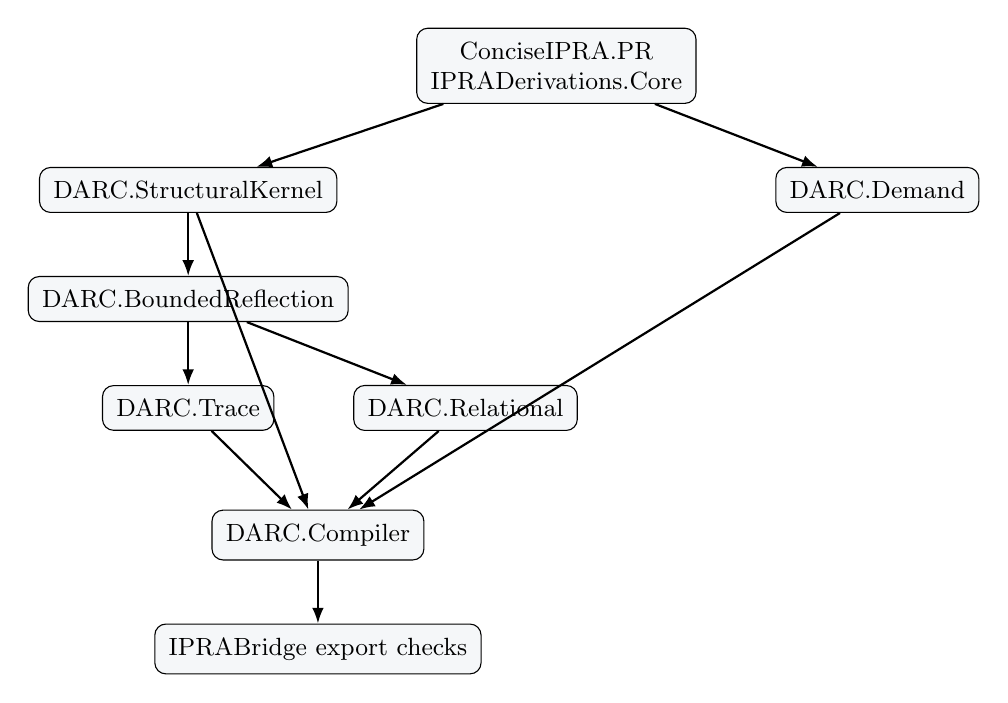
\begin{tikzpicture}[
  node distance=8mm and 10mm,
  box/.style={draw,rounded corners,align=center,fill=darcgray,inner sep=5pt,font=\small},
  arr/.style={-{Latex[length=2mm]},thick}
]
\node[box] (up) {ConciseIPRA.PR\\IPRADerivations.Core};
\node[box,below left=of up] (struct) {DARC.StructuralKernel};
\node[box,below right=of up] (demand) {DARC.Demand};
\node[box,below=of struct] (bool) {DARC.BoundedReflection};
\node[box,below=of bool] (trace) {DARC.Trace};
\node[box,right=of trace] (rel) {DARC.Relational};
\node[box,below right=10mm and -8mm of trace] (comp) {DARC.Compiler};
\node[box,below=of comp] (bridge) {IPRABridge export checks};
\draw[arr] (up) -- (struct);
\draw[arr] (up) -- (demand);
\draw[arr] (struct) -- (bool);
\draw[arr] (bool) -- (trace);
\draw[arr] (bool) -- (rel);
\draw[arr] (demand) -- (comp);
\draw[arr] (trace) -- (comp);
\draw[arr] (rel) -- (comp);
\draw[arr] (struct) -- (comp);
\draw[arr] (comp) -- (bridge);
\end{tikzpicture}
\end{center}

The demand module is metatheory: it proves facts about finite plans and returns
resource states.  The structural, reflection, trace, relational, and compiler
modules construct values of the ordinary \code{Prf PRAAx} type.

\subsection{Structural kernel}

The file \pathcode{lean/DARC/StructuralKernel.lean} contains no
\code{sorry}, \code{admit}, or new \code{axiom}.  It defines:
\begin{itemize}
  \item \code{OpenContract} and \code{openContract\_iff};
  \item context replacement by \code{Prf.trans};
  \item free-variable specialization by \code{Prf.subst};
  \item a scoped certificate structure and sealing by \code{Prf.exE};
  \item a wrapper around \code{Search.search\_found} for named export;
  \item a quantifier-free loop structure and runner using \code{IPRA.ind};
  \item reuse of closed derivations under arbitrary hypotheses.
\end{itemize}
The first formalization step is to place this file in the current Lake
workspace and resolve any namespace or import drift.  Since every proof is a
direct call to a checked API, this step should be small and gives immediate
value even before the full compiler exists.

A representative declaration is:
\begin{lstlisting}[language={}]
def OpenContract (Gamma : List (Fm PTm n)) (A : Fm PTm n) : Prop :=
  forall Delta, (forall C in Gamma, Delta |- [PRAAx] C) ->
    Delta |- [PRAAx] A

theorem openContract_iff :
    OpenContract Gamma A <-> Gamma |- [PRAAx] A := ...
\end{lstlisting}
The actual file uses Lean notation and scoped variables.

\subsection{Demand formalization}

The metalevel demand module should avoid unnecessary abstract lattice
machinery.  Define a shape by capacities \(c_i\), a demand as a dependent
vector of \code{Fin (c i + 1)}, coordinatewise order, join, and rank.  Prove:
\begin{enumerate}
  \item join is an upper bound;
  \item strict coordinatewise increase raises rank;
  \item rank is bounded by the sum of capacities;
  \item inflationary iteration stabilizes within that sum;
  \item monotonicity implies leastness.
\end{enumerate}
For executable plans, a threshold rule can be a finite map from trigger
coordinates to levels and from required coordinates to levels.  A generic
lemma proves its transfer monotone.  More complicated modules may provide a
custom transfer and a monotonicity theorem.

The blueprint \pathcode{lean/DARC/DemandBlueprint.lean} records the intended
signatures.  Its proof milestones are metatheoretic and do not add object
axioms.

\subsection{Bounded reflection}

A robust representation should store atom evidence in the syntax.  One option
is a dependent structure:
\begin{lstlisting}[language={}]
structure ReflectedAtom (n : Nat) where
  bit      : PR n
  formula  : Fm PTm n
  range    : [] |- [PRAAx] bitTerm = 0 or bitTerm = 1
  reflect  : [] |- [PRAAx] (bitTerm = 1 <-> formula)
\end{lstlisting}
The fixed formula syntax then contains \code{ReflectedAtom}, Boolean
connectives, and bounded binders.  The generated \code{bit} and
\code{denote} functions recurse in Lean.  Reflection is proved by induction on
the syntax.  The bounded binder cases should reuse existing finite sums and
products rather than inventing a second arithmetic library.

Binder substitution is the main engineering risk.  The implementation should
first establish reusable lemmas for shifting the generated body symbol and
instantiating it at the bounded index.  Small tests with one free parameter
under two nested binders should precede the strategy compiler.

\subsection{Trace formalization}

A trace specification stores a finite state arity, initial terms, step terms,
and a quantifier-free invariant.  Generate state functions using existing
primitive recursion and pairing/simultaneous recursion.  Prove zero and
successor equations at arbitrary terms.  Then expose a theorem whose inputs
are exactly the base and one-step invariant derivations and whose output is the
open invariant.

Do not encode the invariant as an arbitrary syntax code evaluated at runtime.
It is a fixed \code{Fm PTm} value, and the theorem is generated for it.
Bounded assertions inside the informal invariant must already have been
replaced by reflected bits.

\subsection{Relational formalization}

For a first implementation, use a uniform numerical bound at each layer and a
fixed primitive-recursive edge bit.  Define viability by primitive recursion on
remaining depth, using a finite \code{any} fold.  Prove the one-step theorem:
\[
  V_h(x)=1\to
  \exists y<B_{h+1}\,[E_h(x,y)=1\wedge V_{h+1}(y)=1].
\]
Then use \code{Search.search\_found} to define the least viable successor and
prove the finite path invariant.  General finite coded sets can be added after
this numerical version works.

\subsection{Proof plan and compiler}

The global plan exists in Lean metatheory and stores local theorem values.
Because theorem types depend on node formulas, a fully generic dependent graph
can become cumbersome.  A practical staged implementation is:
\begin{enumerate}
  \item generate one Lean module per concrete plan;
  \item declare node formulas and local proof constants in that module;
  \item generate the topological schedule as ordinary Lean code using
        \code{Prf.trans};
  \item use a generic metatheoretic demand library to decide which declarations
        are emitted;
  \item only later abstract common dependent graph machinery.
\end{enumerate}
This route gives checked application pilots sooner and avoids spending months
formalizing a universal compiler representation before validating the local
interfaces.

The blueprint \pathcode{lean/DARC/CompilerBlueprint.lean} states the ideal
generic theorem, but the generated-module approach is an equally valid path to
a complete checked result.

\subsection{Axiom and dependency audit}

Every completed module should have a check file that:
\begin{enumerate}
  \item imports only the intended lower layers;
  \item prints the exact theorem types;
  \item runs \code{\#print axioms} on exported declarations;
  \item scans for \code{sorryAx};
  \item records the Lake command and repository commit;
  \item checks that the ordinary arithmetic layer does not import application
        endpoints or a second backend unexpectedly.
\end{enumerate}
A theorem is marked checked only after this audit succeeds.  Source files with
no visible placeholders but no elaboration record remain source candidates.

\subsection{Suggested integration milestones}

\begin{description}
  \item[M0.] Elaborate the structural kernel and add axiom checks.
  \item[M1.] Check demand stabilization/leastness and reproduce the JSON
        example in Lean metatheory.
  \item[M2.] Reflect conjunction, disjunction, and one bounded existential;
        then add nested alternation.
  \item[M3.] Prove the square-accumulator trace and a finite viability path as
        ordinary sequents.
  \item[M4.] Generate one concrete proof graph module and compile it by
        simultaneous cut.
  \item[M5.] Export the result through the open Bridge and compare client
        symbols.
  \item[M6.] Migrate one real packet with a nontrivial residual modulus and
        show that discharging the producer removes the boundary.
\end{description}
The detailed commands and acceptance criteria are in
\pathcode{lean/FORMALIZATION_PLAN.md}.

\section{Verification status, limitations, and research program}
\label{sec:status}

A framework of this scope is useful only if its claims are sharply separated.
This section records what the artifact establishes and what remains to be
checked.

\subsection{Established at the human-proof level}

The report gives complete arguments for the following generic conditional
results:
\begin{enumerate}
  \item stabilization and leastness of the finite unified demand analysis;
  \item safe pruning relative to sound transfer summaries;
  \item equivalence of open contracts and ordinary sequents;
  \item acyclic proof-graph compilation by simultaneous cut;
  \item local certificate sealing, stable observation, and bounded named
        export;
  \item fixed bounded-formula reflection from reflected atoms;
  \item soundness of finite positive strategy certificates;
  \item normalized quantifier-free trace reflection;
  \item finite backward viability, least compatible paths, and finite
        observational descent;
  \item guarded quantitative operation interfaces;
  \item the global DARC soundness and relative residual-exactness theorems.
\end{enumerate}
These are theorem schemas: an application must instantiate their stated local
proof obligations.

\subsection{Executable finite evidence}

The reference module \pathcode{reference/darc_reference.py} implements:
\begin{itemize}
  \item finite product-chain demands and threshold rules;
  \item least inflationary closure with a rank bound;
  \item exhaustive monotonicity and leastness checks for small instances;
  \item bounded least search;
  \item positive bounded-formula strategy construction and checking;
  \item deterministic trace execution/checking;
  \item finite backward viability and least paths.
\end{itemize}
The test suite exercises cyclic closure, query-specific liveness, residual
reporting, malformed-rule rejection, strategy tampering, traces, and viable or
nonviable relations.  The generated JSON example records the demand history and
finite certificates.

This code is not an \(\iPRA\) proof checker and is not in the trusted proof
base.  Its role is to test finite algorithms and make the compilation plan
auditable.

\subsection{Lean status}

The structural kernel is written without placeholders and uses current API
names found in the pinned repository.  It was not elaborated here because the
runtime did not contain Lean.  Therefore the artifact does not claim it as a
new checked theorem.  The demand, bounded-reflection, trace, relational, and
compiler files are explicit blueprints containing marked \code{sorry}
milestones.

The theorem ledger in \pathcode{metadata/THEOREM_LEDGER.csv} assigns one of:
fully argued, checked upstream interface, source candidate, Lean blueprint,
executable finite test, or open residual.  No status is inferred from file
names.

\subsection{Deliberate nonclaims}

The artifact does not claim:
\begin{itemize}
  \item a general effective Faltings, Siegel, or Mordell--Weil theorem;
  \item unrestricted exact branch, root, or eigenvector selection;
  \item a global Cauchy modulus from metastability alone;
  \item an infinite path from compatible finite horizons alone;
  \item an effective height bound from qualitative finiteness;
  \item a total universal primitive-recursive evaluator;
  \item that the supplied Lean blueprints compile;
  \item that any new main application theorem is kernel checked.
\end{itemize}
The framework identifies the exact producer interfaces needed by such claims.

\subsection{Research priorities}

The highest-value next step is not another large paper.  It is an integrated
Lean slice that proves one nontrivial endpoint through all layers:
\begin{enumerate}
  \item a fixed bounded formula with alternation;
  \item a loop whose invariant contains the generated truth bit;
  \item a local existential certificate that is sealed;
  \item one named witness selected by checked bounded search;
  \item a cyclic precision demand exposing one residual producer;
  \item a compiled ordinary open sequent;
  \item an open Bridge export to a Foundation client.
\end{enumerate}
Such a pilot would validate the architecture more decisively than separately
elaborating many utility modules.

A second priority is to attach transfer summaries to existing checked
\pathcode{IPRADerivations} lemmas.  The arithmetic library already contains
many proof components; a compact resource interface would make them available
to generated plans without recoding their proofs.

A third priority is producer-driven migration of analytic packets.  Select one
packet whose algebraic and finite parts are mature and whose only missing input
is a clearly stated tail or domain modulus.  Compile the exact conditional
endpoint, then formalize that producer.  This would demonstrate the practical
value of residualization.

\subsection{Conclusion}

DARC turns the broad question ``can this mathematics be expressed in
\(\iPRA\)?'' into a sequence of reviewable obligations:
\begin{enumerate}
  \item What is the exact finite public query?
  \item Which witnesses, precisions, guards, and producers does it force?
  \item Which bounded formulas must be reflected to bits?
  \item Which cycles are finite demand cycles, which are induction loops, and
        which require a genuine extension theorem?
  \item Which local results are ordinary open derivations?
  \item Which deep quantitative inputs remain residual?
\end{enumerate}
The least demand state provides one answer shared by proof scheduling,
certificate escape, precision propagation, and residual exposure.  The final
object is not a semantic promise but an ordinary \(\Prf\;\PRAAx\) derivation.
That combination gives a plausible path from the repository's many rich proof
outlines to a smaller number of reusable, checked, and accurately scoped
formal theorems.

\appendix
\section{Reference algorithms and worked finite instance}
\label{app:reference}

This appendix describes the exact finite algorithms in the artifact.  They are
included for reproducibility and testing, not as a substitute for the Lean
formalization.

\subsection{Demand closure pseudocode}

\begin{lstlisting}[language=Python]
def close(seed, transfer, capacity_sum):
    d = seed
    history = [d]
    for _ in range(capacity_sum + 1):
        nxt = join(d, transfer(d))
        if nxt == d:
            return d, history
        assert rank(nxt) > rank(d)
        d = nxt
        history.append(d)
    raise Error("rank bound violated")
\end{lstlisting}
The implementation validates coordinate names and levels.  For small shapes it
exhaustively checks every admissible candidate to verify leastness.  It checks
monotonicity on every comparable pair when that set is below a configurable
limit; threshold-rule monotonicity is otherwise justified symbolically by the
form of the rules.

\subsection{Strategy checker pseudocode}

For a positive bounded formula:
\begin{lstlisting}[language=Python]
check(atom A, c, env) = (c.tag == atom and A(env))
check(P and Q, c, env) =
    c.tag == and and check(P,c.left,env) and check(Q,c.right,env)
check(P or Q, c, env) =
    c.side selects a branch whose subcertificate checks
check(exists i<N. P, c, env) =
    0 <= c.witness < N and check(P,c.sub,env[i := c.witness])
check(forall i<N. P, c, env) =
    c has N branches and each branch i checks under env[i := i]
\end{lstlisting}
The builder chooses the leftmost true disjunct and least true existential
witness.  These canonical choices model the object-level bounded-search plan.

\subsection{Backward viability pseudocode}

\begin{lstlisting}[language=Python]
viable[H] = terminal layer
for h = H-1 down to 0:
    viable[h] = [x in X[h] | exists y in viable[h+1], edge(h,x,y)]

if start not in viable[0]: fail
path = [start]
for h = 0 .. H-1:
    path.append(least y in viable[h+1] with edge(h,path[h],y))
\end{lstlisting}
The object formalization replaces host lists and predicates by bounded codes,
truth bits, finite folds, and checked least search.

\subsection{Generated demand instance}

The demonstration's public seed requests an approximate value but not a named
witness.  The closure reaches:
\begin{center}
\begin{tabular}{@{}lr@{}}
\toprule
Coordinate & Final level \\
\midrule
query:value & 1 \\
query:witness & 0 \\
cert:branch & 0 \\
cert:trace & 0 \\
precision:root & 5 \\
precision:integral & 6 \\
guard:separation & 0 \\
guard:denominator & 1 \\
residual:tail\_modulus & 1 \\
residual:height\_bound & 0 \\
\bottomrule
\end{tabular}
\end{center}
Thus the generated endpoint needs a denominator guard and tail modulus but not
branch separation, trace replay, or a Diophantine height bound.  This is the
kind of cross-category pruning that motivates the unified lattice.

\subsection{Test inventory}

The eleven unit tests cover:
\begin{enumerate}
  \item a cyclic demand closure;
  \item exhaustive leastness for the small test lattice;
  \item exhaustive monotonicity over comparable pairs;
  \item query-specific certificate liveness;
  \item residual and guard reporting;
  \item rejection of out-of-range rules;
  \item bounded least search;
  \item valid strategy construction;
  \item rejection of a tampered strategy and of a false existential;
  \item deterministic trace checking;
  \item viable and nonviable layered relations.
\end{enumerate}
The build script reruns these tests before compiling the PDF.

\section{Application proof-obligation template}
\label{app:obligations}

A new application should fill the following checklist.  It is designed to keep
mathematical status and compiler status separate.

\subsection{Public theorem}

\begin{enumerate}
  \item State the exact ordinary \(\iPRA\) formula, including free parameters,
        coding conventions, and requested precision.
  \item State whether the endpoint is an open sequent, closed sentence, or a
        backend translation.
  \item Identify every public witness or code that must be named.
\end{enumerate}

\subsection{Representations}

For each mathematical object:
\begin{enumerate}
  \item give its numerical code and primitive-recursive operations;
  \item give validity and equality/compatibility formulas;
  \item specify failed or singular-case conventions;
  \item list checked upstream symbols that are reused;
  \item provide reflection theorems for every atom used in bounded formulas.
\end{enumerate}

\subsection{Plan nodes}

For each node record:
\begin{enumerate}
  \item node identifier and kind;
  \item dependency formulas;
  \item output formula;
  \item local \(\Prf\;\PRAAx\) theorem name or explicit residual status;
  \item certificate scope: none, local, observed, or named;
  \item transfer summary with a human proof of soundness;
  \item imports and replay command.
\end{enumerate}

\subsection{Loops and relations}

For every loop:
\begin{enumerate}
  \item list state registers and step terms;
  \item display the quantifier-free invariant after Boolean compilation;
  \item provide base and step derivations;
  \item provide a fuel or termination-bound theorem.
\end{enumerate}
For every relational cloud:
\begin{enumerate}
  \item state layer bounds and edge bits;
  \item state terminal acceptance;
  \item decide whether the path is local, observed, or named;
  \item state any extension or tail producer separately from finite viability.
\end{enumerate}

\subsection{Quantitative producers}

For every approximation operation:
\begin{enumerate}
  \item state the error predicate;
  \item prove the precision transfer and its monotonicity;
  \item state magnitude, apartness, gap, coverage, and tail requirements;
  \item classify each requirement as checked, to be proved, or residual.
\end{enumerate}

\subsection{Compilation audit}

The generated record should include:
\begin{enumerate}
  \item resource shape, query seed, fixed point, and iteration history;
  \item monotonicity evidence for every transfer;
  \item retained and pruned nodes;
  \item final residual formulas;
  \item exact ordinary endpoint;
  \item theorem names used in the simultaneous-cut schedule;
  \item axiom audit and absence of \code{sorryAx};
  \item backend symbol comparisons and translated endpoint, if any.
\end{enumerate}

\subsection{Status vocabulary}

Use only the following status labels:
\begin{description}
  \item[Checked upstream.] A declaration was built and audited in the pinned
  repository or a recorded compatible baseline.
  \item[Checked in application.] A new declaration was built and audited by
  the application replay.
  \item[Human proof.] A complete nonformal argument is supplied but no Lean
  elaboration is claimed.
  \item[Source candidate.] A no-placeholder source file exists but has not
  been elaborated in the recorded environment.
  \item[Lean blueprint.] Signatures and proof plan exist with explicit
  milestones.
  \item[Executable finite test.] Host code verifies finite examples only.
  \item[Residual.] The exact producer theorem remains an assumption.
\end{description}
This vocabulary prevents a compiled PDF, passing Python test, or no-placeholder
text file from being mistaken for a kernel-checked object theorem.


\begin{thebibliography}{99}
\bibitem{provit-readme}
V. Reshetnikov, \emph{ProveIt: Primitive Recursive Arithmetic}, repository
files under \pathcode{Logic/PrimitiveRecursiveArithmetic}, baseline commit
\texttt{2ef31aa3e313d792df6b63bb28babfe48e1f982e}, 2026.

\bibitem{kleene}
S. C. Kleene, \emph{Introduction to Metamathematics}, North-Holland, 1952.

\bibitem{troelstra}
A. S. Troelstra and D. van Dalen, \emph{Constructivism in Mathematics},
volumes I--II, North-Holland, 1988.

\bibitem{tarski}
A. Tarski, \emph{A lattice-theoretical fixpoint theorem and its applications},
Pacific Journal of Mathematics 5 (1955), 285--309.

\bibitem{cousot}
P. Cousot and R. Cousot, \emph{Abstract interpretation: a unified lattice model
for static analysis of programs}, POPL, 1977.

\bibitem{bishop}
E. Bishop and D. Bridges, \emph{Constructive Analysis}, Springer, 1985.
\end{thebibliography}

\end{document}
